\documentclass[11pt]{article}

% ---------- geometry and fonts ----------
\usepackage[a4paper,left=2.8cm,right=2.8cm,top=2.8cm,bottom=3.0cm]{geometry}
\usepackage[T1]{fontenc}
\usepackage[utf8]{inputenc}
\usepackage{mathptmx}
\usepackage{microtype}

% ---------- maths, tables, figures ----------
\usepackage{amsmath,amssymb,amsthm}
\usepackage{booktabs,threeparttable,graphicx,longtable,array}
\newcolumntype{P}[1]{>{\raggedright\arraybackslash}p{#1}}
\usepackage[font=small,labelfont=bf,skip=6pt]{caption}
\usepackage{setspace}
\usepackage{enumitem}
\setlist{leftmargin=2.2em,labelsep=0.5em,itemsep=2pt,topsep=4pt}
\setlist[enumerate]{leftmargin=2.4em,labelwidth=1.9em,align=left}
\usepackage{titlesec}
\titlespacing*{\paragraph}{0pt}{1.4ex plus .4ex minus .2ex}{0.6em}
\usepackage{fancyhdr}
\PassOptionsToPackage{hyphens}{url}\usepackage[hidelinks]{hyperref}\urlstyle{same}
\hypersetup{pdftitle={The Price of a Design Parameter: Bank Valuations in the Digital Euro Legislative Process},pdfauthor={Philip Kroos}}
\usepackage{natbib}
\bibpunct{(}{)}{;}{a}{}{,}

% ---------- layout ----------
\onehalfspacing
\setlength{\parindent}{1.2em}
\setlength{\parskip}{0pt}
\setlength{\abovedisplayskip}{10pt}\setlength{\belowdisplayskip}{10pt}
\allowdisplaybreaks
\renewcommand{\arraystretch}{1.08}
\captionsetup[table]{position=top}
\captionsetup[figure]{position=bottom}
\theoremstyle{plain}\newtheorem{proposition}{Proposition}
\newcommand{\ph}[1]{\textcolor{red}{[#1]}}
\usepackage{xcolor}

\pagestyle{fancy}
\fancyhf{}
\fancyfoot[R]{\small\thepage}
\renewcommand{\headrulewidth}{0pt}
\renewcommand{\footrulewidth}{0pt}
\fancypagestyle{plain}{\fancyhf{}\fancyfoot[R]{\small\thepage}\renewcommand{\headrulewidth}{0pt}}

\title{\bfseries The Price of a Design Parameter\\[3pt]
\large Bank Valuations in the Digital Euro Legislative Process}
\author{Philip Kroos\\[2pt]\normalsize\href{mailto:philip.kroos@gmx.de}{philip.kroos@gmx.de}}
\date{October 2026}

\begin{document}
\maketitle
\thispagestyle{empty}

\begin{abstract}\noindent\normalsize
The holding limit on the digital euro was designed to prevent deposit flight from banks. We ask whether markets priced the design choices legislators made between 2023 and 2026. We code 22 verified event dates by their available design content before looking at any price, and add the published record of 309 disclosed lobbying meetings. When every event is dated by the day its content became public, the relative gain of a euro area bank one standard deviation more deposit-funded, on an event that limits the digital euro, is $-0.01$ percentage points (placebo-date $p=0.91$); the pre-specified dating, which used the document date of a report already covered by the press, gives 0.05 ($p=0.45$). Allowing for shocks common to all banks on an event day, the estimates exclude effects about a quarter to a third the size of those documented for 2020 and 2021. Events that set a design parameter show no detectable effect. The same design finds a slope close to the 2020 size on the day the Eurosystem report appeared, also with strictly pre-event betas; it is larger in absolute value than 94\% of the slopes on ordinary trading days. Markets appear to have reacted to early news about whether a digital euro would exist; we find no comparable response to later news about its design.
\end{abstract}

\vspace{0.6em}
\noindent\textbf{Keywords:} central bank digital currency; digital euro; financial stability; deposit flight; payments; event study; political economy of regulation.

\vspace{0.3em}
\noindent\textbf{JEL classification:} E42, E58, G21, G28, D72.

\clearpage
\setcounter{page}{1}

\section{Introduction}\label{sec:intro}

The central financial-stability concern about a retail central bank digital currency is deposit flight: households moving balances out of banks into central bank money, gradually or in a run. The holding limit on the digital euro exists to contain that risk. Whether it does so, and whether markets believe it does, depends on how the instrument is designed, and the common description of a CBDC as a simple threat to bank deposits is incomplete in a way that matters for policy. The digital euro, as it has actually been drafted, is a bundle of parameters: a ceiling on how much any person may hold, a rule on whether firms may hold at all, a cap on what merchants and payment providers may charge each other, a mandate that device manufacturers open their hardware, and a decision on whether an online version is built at all. Each parameter moves rent from one part of the payments chain to another. The aggregate effect on banks is the sum of these transfers, and it can be positive or negative depending on how the parameters are set.

This distinction is not academic. Between June 2023 and July 2026 the European Parliament and the Council did not debate whether to have a digital euro. They debated the parameters. The rapporteur's draft report of November 2025 proposed that the online version be built only if the Commission first concluded that no private pan-European alternative exists. The Council's position of December 2025 capped interchange and merchant fees for at least five years and required device manufacturers to grant access to their hardware. The committee position of June 2026 barred firms from holding digital euro beyond twenty-four hours. Each of these is a transfer with a price, and the prices are not known.

\paragraph{This paper.} We measure what a design parameter is worth, and to whom. The empirical design is a two-stage event study over the legislative phase. In the first stage we compute abnormal returns for the 49 listed firms with usable price data, 29 of them euro area banks, from factor models appropriate to the market of listing. In the second stage we relate them to firm exposure interacted with the coded design content of each event, with firm and event fixed effects, so that everything common to a trading day is absorbed and identification comes from the cross-section.

\paragraph{What makes the design work.} The events are not one-dimensional. The same announcement can be good news for banks and bad news for payment providers, because it limits quantities and caps fees at the same time. Figure~\ref{fig:timeline} and Table~\ref{tab:events} show the coded pattern: the committee position and its confirmation in plenary carry opposite signs for banks and payment providers, and several other events move one group while leaving another untouched. The coding predicts that such an announcement raises one group and lowers another, which a common news-intensity channel could not produce. Whether the prediction holds is an empirical question, and Section~\ref{sec:results} shows that for payment providers it mostly does not. The two-sided coding is what separates our design from an event study of project news, and it is the reason we code content before seeing prices. The coefficient it delivers is the valuation response to a decision of a given direction, not the value of one more euro of holding limit: the coding records the direction of each act, not its size in euro.


\begin{figure}[t]\centering
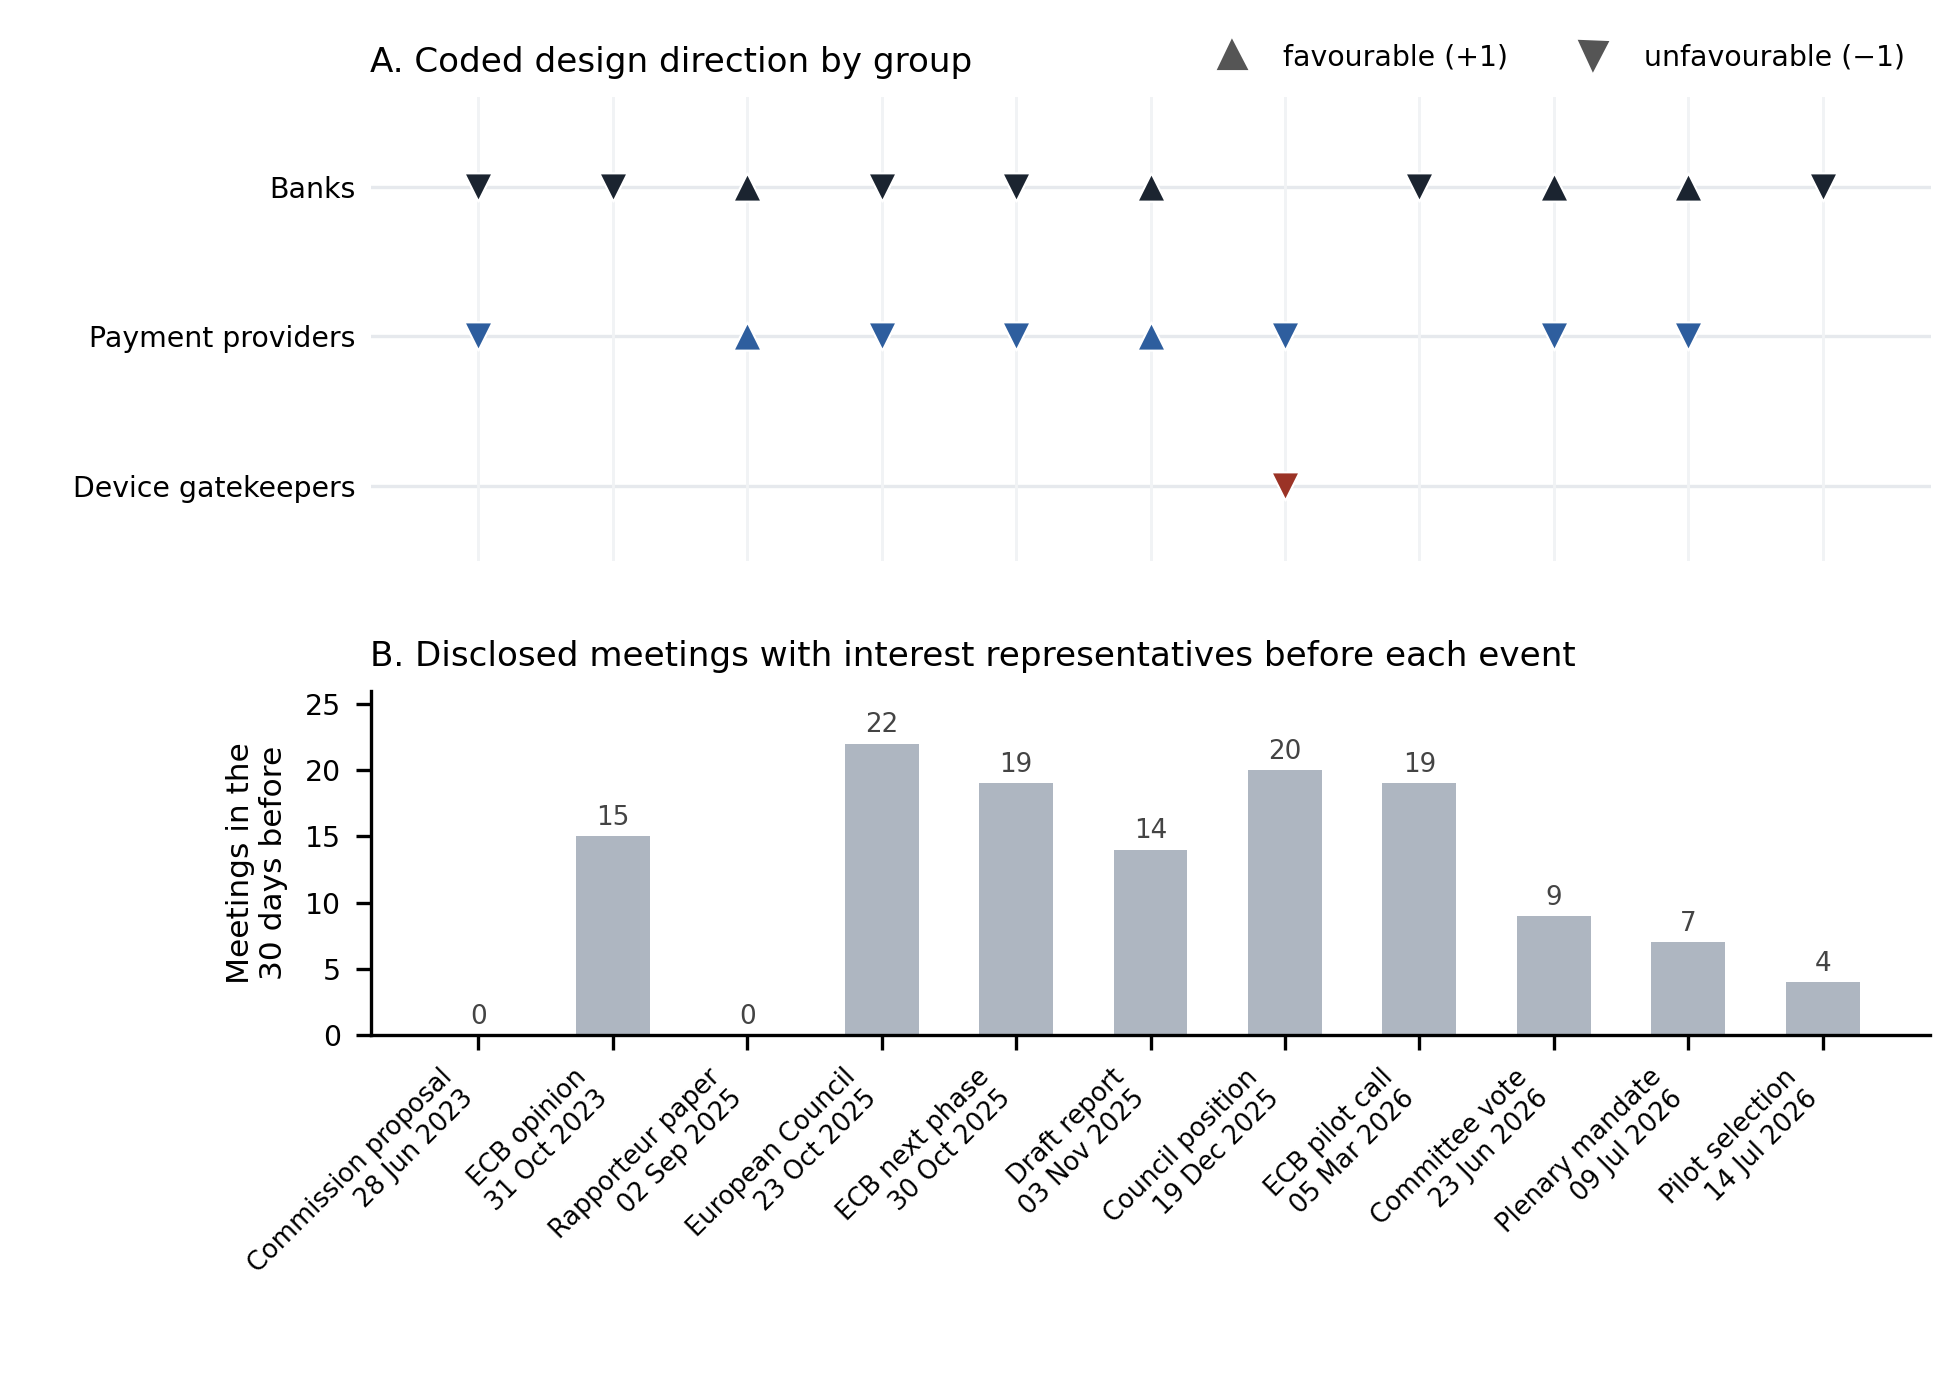
\includegraphics[width=\textwidth]{figures/fig_timeline.png}
\caption{The digital euro file: contestation and coded design content}\label{fig:timeline}
\par\vspace{2pt}\begin{minipage}{\textwidth}\footnotesize\textit{Notes:} Events with a non-zero coded direction for at least one group, in chronological order. Direction is coded from the contemporaneously available text of the act before any price data was loaded; groups coded zero for an event are left blank. Panel B counts meetings disclosed on procedure file 2023/0212(COD) by rapporteurs, shadow rapporteurs and the committee chair in the 30 calendar days before each event. The draft report is shown at its document date of 3 November 2025; the preferred estimates date it by the first trading day after its content was reported, 31 October 2025.\end{minipage}
\end{figure}

\paragraph{A second, independent source.} The European Parliament publishes every meeting between rapporteurs, shadow rapporteurs, committee chairs and interest representatives on the procedure file. We transcribe the complete published record: 309 disclosed meetings between July 2023 and July 2026, with date, member, role and organisation. Deutsche Bank appears twelve times, the French banking federation ten, Amazon and the European consumer organisation eight each, Banco Santander seven. This record serves three purposes. It documents which interests bargained over which parameter. It provides a measure, observable before the event, of how contested each step was, which speaks to the anticipation critique that event studies of legislation usually face. And it validates the falsification events from outside the price data: exactly one meeting precedes the purely procedural event of November 2024, against twenty-two in the thirty days before the Eurogroup agreement on the holding-limit mechanism.

\paragraph{What we find.} The legislative design of the digital euro moved bank valuations little, if at all. We date every event by the day its content became public. For one event this differs from the pre-specified dating: the content of the rapporteur's draft report was first reported after the close of European markets on 30 October 2025, so that it reached prices on 31 October, one trading day before the date on the document. In this preferred specification, the relative gain of a euro area bank one standard deviation more deposit-funded, on an event that limits the digital euro, is $-0.01$ percentage points, with a permutation $p$-value of 0.89 and a placebo-date $p$-value of 0.91. The pre-specified dating gives 0.05 ($p = 0.45$); we report it throughout as the reference. Banks share shocks on any given day, so we draw inference at the level of events as well as firms. With standard errors that allow for such shocks, the 95\% confidence interval of the preferred estimate runs from $-0.29$ to $0.26$ percentage points per standard deviation, and that of the pre-specified estimate from $-0.23$ to $0.33$. Both exclude effects of the size that \citet{burlon2024} document for the ECB's announcements of 2020 and 2021, more than one percentage point per standard deviation, and the preferred estimate excludes effects about a quarter that size. Aligning every event to its documented release time, with two-day windows for the eleven releases whose time of day is not documented, gives 0.03 to 0.05 percentage points depending on the return benchmark, with permutation $p$-values between 0.61 and 0.77. An earlier version of this alignment, which treated the draft report and the ECB release of the same week as undocumented, gave 0.15 to 0.17 with permutation $p$-values between 0.05 and 0.12; Section~\ref{sec:flow} shows that the difference comes entirely from attributing the market's reaction to the draft report to the wrong event. In a decomposition we added after the pre-specified analysis, the events that fixed a design parameter, as distinct from events that only changed the likelihood of issuance, show no detectable effect in any event window. Contested and unscheduled events show nothing, which speaks against anticipation, and the same exposure slope appears for banks outside the euro area, which is consistent with a generic factor loading on deposit-funded banks rather than a digital-euro-specific response. Payment providers show no consistent response, and the response of device gatekeepers rests on a single event; our evidence on the non-bank side of the payments chain is correspondingly weaker than on banks, and the paper's empirical claims concern banks first.

The null is not a failure of the design to see anything. Extending the sample to 2020 and 2021 with the same firms, exposure measure and estimator, the design finds a slope of 0.85 percentage points per standard deviation, with exposure measured before the event, on the day the Eurosystem published its report on a digital euro, close to the magnitude documented in the earlier literature. It is a single day, and it lies at the edge of what ordinary days produce: 94\% of the slopes on trading days of 2019 to 2021 without digital euro news are smaller in absolute value. What it does not detect, in 2021 or later, is any response to news about how the instrument would be designed, including the first signal of a holding limit in February 2021. The market appears to have reacted to early news about whether a digital euro would exist; we find no comparable response to news about its design.

\paragraph{Why it matters.} Two conclusions follow for policy. For financial stability, markets did not assign a large residual deposit-flight risk to euro area banks during the legislative process: any effect on banks with very different exposure appears modest relative to the response to the early digital euro announcements. The parameters that took three years to negotiate were, in the market's assessment, second order to bank value. This is consistent with the simulation evidence of \citet{meller2023}: the limits under discussion, up to EUR 3,000 per person, are within the range for which they find contained effects on bank liquidity and funding. For the political economy of the file, the negotiation record shows that the same parameters were intensely contested, with the banking side the most frequent counterparty of the legislators. The contrast between what was bargained over and what was priced is itself informative: whatever the banks were negotiating for did not generate a large detectable valuation response in equity markets.

\paragraph{Related literature.} The paper connects to five literatures.

\textbf{CBDC and bank intermediation.} The canonical concern is that a central bank liability available to households substitutes for deposits and shrinks the funding base of banks. \citet{brunnermeier2019} show conditions under which the substitution is neutral, because the central bank can pass the funds back to banks; \citet{fernandezvillaverde2021} show that a CBDC may concentrate deposits at the central bank in a run; \citet{andolfatto2021} shows that a CBDC can raise deposits when banks have market power. \citet{keister2023} formalise the trade-off between more efficient exchange and crowded-out deposits, with an optimum that depends on how valuable bank intermediation is at the margin. \citet{chiu2023} add imperfect competition and overturn the sign: with deposit market power, which is large in the data \citep{drechsler2017}, a CBDC forces deposit rates up and can \emph{raise} deposits and lending. The empirical question is therefore not whether a CBDC hurts banks but where in the cross-section it hurts and by how much. Our design speaks directly to the cross-sectional question and only indirectly to the level.

\textbf{Quantity limits as the policy instrument.} Because the sign of the intermediation effect is ambiguous, the policy debate has concentrated on bounding the quantity. \citet{bidder2024} distinguish slow deposit substitution in normal times from fast disintermediation during banking stress and show in their calibrated model that a suitably chosen holding limit can contain the run-risk channel. The European negotiation uses a standing ceiling reviewed on a fixed cycle, so our events speak to the quantity channel rather than directly to run dynamics. For the euro area, \citet{meller2023} simulate a digital euro with supervisory data on more than 2,000 banks and find that a EUR 3,000 per-person holding limit would have contained effects on bank liquidity risks and funding structures even in extremely pessimistic scenarios. \citet{lambert2024} likewise assess safeguards designed to limit effects on bank liquidity and central-bank reliance. \citet{munoz2023} study the demand for public money as a store of value when beliefs are heterogeneous. \citet{auer2025} provide further simulation evidence on the banking system, and \citet{chapman2023} survey the literature on CBDC and banking. This work is model-based and simulates the balance-sheet consequences of given limits. Our contribution is the market's own assessment of the limits actually negotiated.

\textbf{Event studies of CBDC news.} \citet{burlon2024} are closest to us and provide the benchmark for magnitudes. They show that news about the digital euro moved euro area bank valuations, scaled by each bank's deposit ratio, with more than one percentage point of abnormal return per standard deviation of the deposit ratio and event, and they connect the valuation effects to lending through credit register data. Their events are communications by members of the ECB's Executive Board in 2020 and 2021, and the sample ends in May 2021. They observe that the trend reverses after the Executive Board first floated a holding limit of EUR 3,000 in February 2021, which is the mechanism we make systematic. \citet{berg2024} study digital euro announcements for payment firms: valuations of US payment firms fall and those of European payment firms rise, while bank stocks do not react significantly. We differ from both in three ways. Our events are legislative and cover the period in which the co-legislators adopted and narrowed their positions on the design parameters. We code each event by its design content for each group rather than treating it as homogeneous news. And we test incidence channel by channel: the fee channel applies two-sided-platform logic \citep{rochet2003} to a regulated new rail, and the device-access provisions operate one layer further down, at the hardware interface.

\textbf{Political economy of financial regulation.} Our negotiation record connects to work on how competing interest groups shape financial legislation \citep{kroszner1998}, on lobbying by financial institutions before the global financial crisis \citep{igan2012}, and on what lobbyists supply to legislators \citep{bertrand2014}. Our reading of the record is deliberately modest. It shows which interests were present and when, which is informative about the contestation of each parameter, but presence is chosen by the interested party and is therefore endogenous to expected exposure. We use the record to validate the coding and to measure contestation, not as a source of variation.

\textbf{Event-study methods.} We build on event studies of regulatory news \citep{schwert1981,binder1985,mackinlay1997}. With few effective clusters and cross-sectionally correlated abnormal returns \citep{kolari2010}, we rely on permutation inference over exposure within groups and a null-imposed wild cluster bootstrap \citep{cameron2008}, and we assess finite-sample size by simulation.

\paragraph{Contribution.} We provide the first event-study use of the digital euro's legislative process to construct parameter-specific design events and measure their incidence across the payments value chain. We also contribute two reusable public-data objects: a primary-source event list with documented design content, and the complete negotiation record of the procedure file.

\section{Institutional background}\label{sec:inst}

\subsection{What the digital euro is, as drafted}

The Commission proposed the regulation establishing the digital euro on 28 June 2023, as document COM(2023)\,0369. The instrument as drafted has four features that determine its economic incidence.

\textbf{It is a liability of the central bank, distributed by intermediaries.} Payment service providers open and service digital euro accounts; the ECB issues the claim. Banks therefore face the substitution of a funding instrument and simultaneously acquire a distribution role.

\textbf{Holdings are capped.} Individual holdings are subject to a limit whose level was left to be decided. At the request of the co-legislators, the ECB later analysed hypothetical limits of EUR 500 to EUR 3,000 under business-as-usual and flight-to-safety scenarios \citep{ecb2025}. \citet{lambert2024} analyse how holding limits can contain effects on bank liquidity and central-bank funding. The limit is the single parameter that determines how much deposit substitution is possible, and it was the most heavily contested item in the file.

\textbf{It carries no interest.} Remuneration is excluded by design, which caps the attractiveness of the instrument as a store of value and distinguishes it from the wholesale CBDC literature.

\textbf{Its fee structure is regulated.} What merchants pay, and what providers may charge each other, is set in the regulation rather than by the market. This is where the incidence for payment providers is determined, and it is economically distinct from the deposit channel.

\subsection{The legislative process as a sequence of parameter decisions}

The file passed through the Parliament and the Council between 2023 and 2026. Table~\ref{tab:events} lists the events we use. Three deserve description because they carry most of the design content.

\textbf{The rapporteur's draft report, 3 November 2025, first reported on 30 October.} After the change of rapporteur in December 2024, the new draft splits the instrument. The offline digital euro, a tokenised device-to-device instrument with cash-like properties, is introduced immediately. The online version, which is the deposit-substituting one, is introduced only if the Commission, after an investigation phase, concludes that no suitable pan-European sovereign retail payment solution exists. Holding limits are made more prescriptive. This is the most quantity-limiting proposal in the file, and it also makes the project conditional on the failure of private European alternatives.

\textbf{The Council position, 19 December 2025.} Limits are set by the ECB but must respect an overall ceiling agreed by the Council and reviewed at least every two years, which moves control of the parameter from the central bank to the legislators. Providers may not charge consumers for mandatory services. A framework guarantees providers access to the hardware and software of mobile device manufacturers. Interchange and merchant service charges are capped for a transitional period of at least five years at levels based on comparable means of payment, and are cost-based thereafter.

\textbf{The committee position, 23 June 2026, confirmed in plenary on 9 July 2026.} An overall cap on holdings is to be set by the Commission on the ECB's recommendation and reviewed at least every two years. Legal persons may not hold digital euro as a general rule and may accumulate incoming payments for at most twenty-four hours. The rollout phase is to last at least twenty-four months. Merchant and inter-provider fees are capped, and offline payments are free of charge.

\subsection{The Commission baseline}

The proposal of 28 June 2023 sets the baseline against which the two positions in Table~\ref{tab:positions} are amendments. Five features of it matter for incidence.

\textbf{Legal tender.} The digital euro is granted legal tender status within the euro area, with Member States designating authorities to enforce acceptance. Acceptance is therefore not a commercial decision, which is what makes the fee provisions binding rather than indicative: merchants cannot decline the instrument and negotiate the price of accepting it.

\textbf{Online and offline, not programmable.} The instrument is available in both forms and is convertible at par with cash and with commercial bank money. Non-programmability was a condition set by finance ministers before the proposal and is preserved in it.

\textbf{Distribution by payment service providers.} All EU providers may distribute, which the Commission underpinned with a parallel regulation for providers incorporated outside the euro area (COM(2023)368) and with the revision of the payment services framework (COM(2023)366) that extends the definition of funds to retail central bank money. Distribution is an obligation for credit institutions in respect of their own customers rather than an opportunity they may decline.

\textbf{Quantitative limits as a financial stability tool.} The proposal states that unrestricted use as a store of value could endanger financial stability and reduce credit provision, and that the ECB may introduce limits, including quantitative limits on individual holdings and limits on conversion. The level is not fixed in the proposal. This is the origin of the parameter that the Parliament and the Council then fought over for three years, and it is why the file is a natural experiment in the pricing of a design choice rather than of a policy announcement.

\textbf{A package, not a single act.} The proposal came with a regulation on the legal tender of cash (COM(2023)364), which is why the Council's December 2025 position covers both the digital euro and the acceptance of cash. Events that touch the cash regulation affect retailers and cash handlers and not banks, which is a further source of cross-sectional variation we code but do not rely on.

\paragraph{A note on dating the Council position.} The Council working document carries 17 December 2025 and the press release announcing the position carries 19 December 2025. We use the press release date, because that is when the substance became public, and report the alternative date in Table~\ref{tab:robust}.

\subsection{The two positions in detail}

By July 2026 the two co-legislators had adopted positions that differ on every parameter that matters for incidence. Table~\ref{tab:positions} sets them side by side. Both are verified from the primary documents: the Council press release of 19 December 2025 and the committee report tabled on 26 June 2026 and confirmed in plenary on 9 July 2026.

\begin{table}[t]\centering\small
\begin{threeparttable}
\caption{The two co-legislator positions on the parameters that determine incidence}\label{tab:positions}
\begin{tabular}{P{3.4cm}P{5.2cm}P{5.2cm}}
\toprule
Parameter & Council, 19 December 2025 & Parliament, 23 June / 9 July 2026 \\
\midrule
Who sets the holding limit & ECB sets limits, but must respect an overall ceiling agreed by the Council, reviewed at least every two years & Commission sets the overall cap on the ECB's recommendation, reviewed at least every two years \\
Holdings by legal persons & Not specified in the press release & As a rule not permitted; incoming payments may be held at most 24 hours before being swept \\
Consumer fees & Providers may not charge for mandatory services; added-value services may be priced & No account maintenance, inactivity or minimum balance fees for basic services; practices circumventing free basic services prohibited \\
Merchant and interchange fees & Capped for a transitional period of at least five years at levels based on comparable means of payment; cost-based thereafter & Capped; offline payments free of charge \\
Access to mobile devices & Framework guaranteeing providers access to the hardware and software of device manufacturers & Not the central instrument in the committee text \\
Rollout & Not specified in the press release & Rollout phase of at least 24 months after authorisation, preceded by pilot testing \\
Liability and privacy & Not specified in the press release & Users bear no losses from outages; the ECB has no access to personal identification data under any circumstances \\
\bottomrule
\end{tabular}
\begin{tablenotes}\footnotesize
\item \textit{Notes:} Entries are taken verbatim in substance from the two primary documents. ``Not specified in the press release'' means the item is not covered in the source we verified and not that the position is silent; the consolidated texts will resolve these cells. The comparison is the object of the interinstitutional negotiations that followed the plenary mandate of 9 July 2026.
\end{tablenotes}
\end{threeparttable}
\end{table}

Three observations follow, and each maps to a channel in Section~\ref{sec:model}.

\textbf{Control over the quantity parameter moved away from the central bank in both positions, but to different bodies.} The Council reserves the ceiling to itself; the Parliament gives it to the Commission on the ECB's recommendation. Either way the parameter that determines deposit substitution became a political variable, reviewed on a two-year cycle. For banks this is favourable relative to unconstrained central bank discretion, because the ceiling is now set by bodies that are directly exposed to their representations, and the negotiation record shows that they made them.

\textbf{The fee provisions bind providers, not banks.} Capping merchant and inter-provider charges transfers rent to merchants. Banks are affected only through their distribution income, which is second order relative to the deposit channel. This is what makes the December 2025 and June 2026 acts two-sided.

\textbf{The device-access provision has one addressee.} Requiring manufacturers to open hardware and software interfaces to payment providers is directed at firms that control a mobile operating system. The record shows two meetings between the rapporteur or a shadow rapporteur and the largest such firm, in November 2025, three weeks before the Council fixed its position, and in June 2026, a week before the committee vote.

\subsection{Why the market could price these events}

Three conditions have to hold for an event study to be informative here, and all three are satisfied.

First, the acts are public on the day. Committee votes, plenary results, Council press releases and ECB publications are dated, and the substantive content is in the release rather than in a consolidated text published weeks later. The time of day is documented for some releases and not for others; Section~\ref{sec:flow} explains how we treat that.

Second, the amounts are large enough to matter for valuations. Euro area overnight deposits of households and non-financial corporations are of the order of several trillion euro, and a holding limit of EUR 3,000 applied to a few hundred million residents defines a substitution capacity in the high hundreds of billions. Whether take-up would approach that capacity is precisely the uncertainty the limit resolves.

Third, the affected firms are listed and the exposure is measurable from public reporting. That is not true of every regulatory file, and it is what makes this one usable.

\subsection{The 2024 standstill and what it implies for coding}

The file did not progress in 2024, and the reason is documented rather than inferred. The draft report tabled by the first rapporteur on 9 February 2024 was never put to a vote. In mid-2024 three shadow rapporteurs wrote to the committee chair complaining that the rapporteur had delayed the process from the start. In December 2024 the rapporteur stepped down and was replaced.

What this implies for coding requires care. In the pre-specified coding the draft of February 2024 and the amendments tabled on it were coded as carrying no design direction, and part of the justification was that the draft was never voted. That justification uses information the market did not have on the day: in February 2024 nobody knew that the draft would stall. The correct question is what a market participant could learn from the text on the day it was published. Because we were unable to retrieve the text of the draft, we cannot answer that question from its content, and the correct treatment is to exclude both events rather than to code them as neutral. We report the pre-specified estimate and the estimate without them; since both carried a zero direction, the change affects only the fixed effects and, as Section~\ref{sec:referee} shows, leaves the result unchanged.

The negotiation record is consistent with a file that stalled in 2024: documented meetings fall from 48 in 2023 to 20 in 2024 and rise to 161 in 2025. We use this only as description, not as a reason for any coding decision.

\paragraph{The change of rapporteur.} At the date of appointment, December 2024, the successor had no publicly documented position on the file. The paper in which he argues that the digital euro is not the answer to European dependence on non-European card networks appeared only in 2025. We therefore code the appointment itself as carrying no direction, and treat the later publication of his position, on 2 September 2025, as a separate event. Coding the appointment as bank-favourable because of what the appointee later wrote would be using information the market did not have.

\paragraph{A note on dating the draft report.} The draft report carries 3 November 2025 and was presented to the committee on 5 November 2025. Its content was public earlier. Bloomberg reported the conditional online version, from the statement accompanying the report, at 21:12 UTC on 30 October 2025, after the close of European markets; the first trading day with the information is therefore 31 October 2025. Dating the event on 31 October applies the rule we use for every other event: the Council position, for instance, is dated by its press release because that is when the substance became public. Our preferred estimates therefore use 31 October 2025. The pre-specified coding used the document date, because we identified the earlier report only after the pre-specified analysis; we report the pre-specified estimates throughout as the reference, and the presentation date in Table~\ref{tab:robust}.

\subsection{The rapporteur's revealed position}

One event in the sample is neither a legislative act nor a central bank decision. On 2 September 2025 the rapporteur published a twenty-seven page chapter in a yearbook on the euro, arguing that the digital euro is not needed and pointing instead to private European alternatives, naming the European Payments Initiative. He presented the piece as a personal contribution rather than as the rapporteur's position.

We include it and code it as favourable for banks and for private European payment schemes, for three reasons. The substance reappeared two months later in his draft report, where the online digital euro is made conditional on the absence of a private pan-European solution and the assessment is assigned to the Commission rather than to the ECB. The author is the single member with agenda control over the file. And the framing as personal does not change what a market participant learns from it, which is the direction in which the file will be steered.

The disclaimer is nevertheless recorded, and the event is included in the leave-one-out set so that the main estimate can be read with and without it.

\subsection{The parallel operational track}

The ECB ran its own timetable alongside the legislature. The preparation phase closed on 30 October 2025 and the project moved to its next phase. A call for expression of interest for pilot participants was published on 5 March 2026 and closed on 14 May 2026; on 14 July 2026 the ECB selected 36 payment service providers from more than 50 applicants, covering banks and non-banks. A call for merchants followed on 15 September 2026. A twelve-month pilot is planned for the second half of 2027, and first issuance is possible in 2029 if the regulation is adopted in 2026.

This track matters for identification in two ways. It produces events that advance the project without changing its design, which are useful as a contrast to design events. And the selection of pilot participants is, in principle, a within-group event: it separates providers that will participate from those that will not, on a single day.

\section{Conceptual framework}\label{sec:framework}

We do not need a full model to sign the empirical predictions. What we need is an accounting of where rent sits in the payments chain and how each parameter moves it.

Consider three incumbent groups. Banks earn a spread $s$ on their deposit base $D_i$, and they also earn fees from distributing payment services. Payment providers, including card networks and acquirers, earn a margin $m$ on their transaction volume $V_j$. Device gatekeepers earn a rent $r$ on each unit of mobile payment volume $V^{\mathrm{mobile}}$ routed through the hardware interface they control.

A digital euro with holding limit $L$, a rule $\lambda\in\{0,1\}$ on whether legal persons may hold it, a fee cap $\bar f$, and a device-access mandate $a\in\{0,1\}$ changes these as follows.

\textbf{The holding limit is the deposit channel.} Substitution away from deposits is bounded by $L$ times the number of users for whom the limit is not slack. A higher $L$ therefore lowers bank rent, and by Proposition~\ref{prop:conc} the marginal loss is larger for banks with a larger fraction of depositors whose balances exceed the limit, since only those depositors can move more when the limit is raised. This is the channel \citet{burlon2024} measure and the one \citet{chiu2023} argue may reverse under imperfect competition, because the threat of substitution forces banks to raise deposit rates only where they previously exercised market power.

\textbf{The rule for legal persons scales the same channel.} Barring legal persons from holding removes corporate balances from the substitutable base entirely.

\textbf{The fee cap is a separate channel that runs through providers, not banks.} A binding cap $\bar f$ transfers rent from providers to merchants without touching deposits. It is possible, and in the committee position of June 2026 it is the case, for one act to limit the deposit channel and tighten the fee channel at the same time.

\textbf{The device-access mandate is a third channel with a single addressee.} Mandated access to hardware dissipates the gatekeeper's rent $rV^{\mathrm{mobile}}$ and passes part of it to providers.

Three predictions follow and are taken to the data.

\begin{enumerate}\itemsep2pt
\item[P1] Events that limit quantity raise bank valuations, and the effect scales with the share of deposits that are potentially substitutable.
\item[P2] Events that cap fees lower the valuations of payment providers, and the effect scales with the share of revenue earned in euro area transactions.
\item[P3] Events that mandate device access lower the valuation of gatekeepers and raise that of providers.
\end{enumerate}
\noindent Prediction P3 is the sharpest, because the addressee is essentially unique. Predictions P1 and P2 are the ones that generate opposite signs on the same day, which is the feature the design rests on.

\section{A model of rent incidence in the payments chain}\label{sec:model}

The purpose of the model is narrow: to derive which group gains and which loses from each design parameter, so that the empirical coding is a prediction rather than a judgement call. It is a static model of a payments market with three incumbent groups and one entrant, the central bank.

\subsection{Environment}

A unit mass of households holds transaction balances $b$, distributed with cumulative distribution $F$ on $[0,\bar b]$. Households make payments of total value $V$. There are three incumbents.

\textbf{Banks} take deposits and earn a spread. Bank $i$ holds deposits $D_i = \int_0^{\bar b} b \, dF_i(b)$ and earns $s\,D_i$, where the spread $s$ is the difference between the market rate and the deposit rate it pays. Banks differ in $F_i$: some have deposit bases concentrated in small transaction balances, others in large ones.

\textbf{Payment providers} process transactions. Provider $j$ handles volume $V_j$ and earns a margin $m$ per unit, so revenue is $m V_j$. The margin has two components, an interchange fee received from the acquiring side and a merchant service charge.

\textbf{Device gatekeepers} control the hardware interface through which mobile payments are initiated. A gatekeeper earns $r$ per unit of volume routed through its interface, either as an explicit fee or as the shadow value of excluding competitors.

The central bank issues a digital euro characterised by four parameters:
\begin{itemize}[leftmargin=2.2em,labelwidth=1.4em,align=left,itemsep=1pt]
\item[$L$] the holding limit per person;
\item[$\lambda$] an indicator, $\lambda\in\{0,1\}$, for whether legal persons may hold;
\item[$\bar f$] a cap on the fees providers may charge;
\item[$a$] an indicator, $a\in\{0,1\}$, for whether device access is mandated.
\end{itemize}

\subsection{Substitution and its bound}

A household substitutes from deposits into digital euro up to $\min(b, L)$. Aggregate substitution from bank $i$ is therefore
\begin{equation}\label{eq:sub}
S_i(L) \;=\; \sigma \int_0^{\bar b} \min(b, L)\, dF_i(b),
\end{equation}
where $\sigma \in [0,1]$ is the take-up rate. Two properties of \eqref{eq:sub} drive everything that follows.

\begin{proposition}[Concavity of substitution in the limit]\label{prop:conc}
$S_i(L)$ is increasing and concave in $L$, with $S_i'(L) = \sigma\,[1 - F_i(L)]$. The marginal effect of raising the limit is therefore proportional to $1-F_i(L)$, the fraction of the bank's depositors whose balances exceed $L$, and it falls to zero as $L$ approaches $\bar b$.
\end{proposition}

Proposition~\ref{prop:conc} has an immediate empirical implication that distinguishes our design from a linear one: the same increment in $L$ is worth more when $L$ is low, and worth more to a bank whose deposits sit in large balances. It also means that a cap set well above the typical transaction balance is close to no cap at all, which is why the debate between EUR 500 and EUR 3,000 was economically substantive rather than symbolic.

\begin{proposition}[Exposure ordering]\label{prop:order}
Let banks $i$ and $k$ have deposit distributions with $F_i$ first-order stochastically dominated by $F_k$. Then $S_i(L) \le S_k(L)$ for every $L$. The level gap $S_k(L)-S_i(L)$ is weakly increasing in $L$, and the difference in marginal effects, $S_k'(L)-S_i'(L)=\sigma[F_i(L)-F_k(L)]$, is largest where the two distribution functions differ most.
\end{proposition}

Two implications matter for measurement. The \emph{level} of substitution a bank faces at a given limit rises with its substitutable deposit base, which motivates a deposit share as the exposure measure. The \emph{marginal} effect of changing the limit depends on the fraction of depositors with balances above the limit, which would require account-level balance distributions that are not public. Our measures therefore capture the first implication directly and the second only by proxy.

\subsection{The three channels}

Bank $i$'s rent is $\Pi^B_i = s\,[D_i - S_i(L) - \lambda C_i] + \phi_i$, where $C_i \ge 0$ are the corporate deposit balances that would move into digital euro if legal persons were permitted to hold it, and $\phi_i$ is distribution income from servicing digital euro accounts, which is bounded by the fee regulation. Provider $j$'s rent is $\Pi^P_j = \min(m, \bar f)\, V_j + a\,\rho_j\, r\, V^{\mathrm{mobile}} - c_j$, where $\rho_j \ge 0$, with $\sum_j \rho_j \le 1$, is the share of the gatekeeper's rent that provider $j$ captures when access is mandated. The gatekeeper's rent is $\Pi^G = (1-a)\, r\, V^{\mathrm{mobile}}$. Whether the dissipated rent reaches providers, and how much of it, is an assumption embodied in $\rho_j$; with $\sum_j\rho_j<1$ part of it is competed away to users.

Differentiating gives the three predictions the empirical work tests.

\begin{proposition}[Quantity channel]\label{prop:quantity}
$\partial \Pi^B_i / \partial L = -s\,\sigma\,[1-F_i(L)] \le 0$, strictly negative whenever $F_i(L)<1$, and $\partial \Pi^B_i / \partial \lambda = -s\,C_i \le 0$, strictly negative when $C_i>0$. Events that lower the limit or bar legal persons raise bank rent, and the effect is proportional to $1 - F_i(L)$.
\end{proposition}

\begin{proposition}[Fee channel]\label{prop:fee}
$\partial \Pi^P_j / \partial \bar f = V_j \cdot \mathbf{1}\{\bar f < m\} \ge 0$. A tighter cap lowers provider rent in proportion to euro area volume, and leaves bank deposit rent untouched except through $\phi_i$.
\end{proposition}

\begin{proposition}[Access channel]\label{prop:access}
$\partial \Pi^G / \partial a = -r\,V^{\mathrm{mobile}} < 0$ and $\partial \Pi^P_j / \partial a = \rho_j\, r\, V^{\mathrm{mobile}} \ge 0$. The access mandate lowers gatekeeper rent unambiguously; it raises provider rent to the extent that $\rho_j>0$; and it has no first-order effect on bank deposit rent.
\end{proposition}

\subsection{Why the signs can differ within one act}

Propositions~\ref{prop:quantity} to \ref{prop:access} operate through different arguments of different rent functions. An act that lowers $L$ and tightens $\bar f$ raises $\Pi^B$ and lowers $\Pi^P$ simultaneously. The committee position of June 2026 has this form: it limits quantities and caps fees. The Council position of December 2025 is more complex. For banks it combines a political ceiling on holdings, which is favourable, with free basic services and capped compensation, which are costly, and we code its net bank direction as zero. For payment providers it combines a fee cap, which lowers their rent, with mandated device access, which raises it when $\rho_j>0$; the model does not sign the net effect without an assumption on the relative size of the two channels. We code it as unfavourable, on the reading that the fee cap applies to all providers while access benefits only those that use it, and we report the provider estimate with this event recoded to zero. The empirical design exploits acts with opposite signs across groups, because a confound would have to be correlated with bank exposure and provider exposure with opposite signs on the same day.

\subsection{What the model does not deliver}

Three limitations are worth stating before the empirical work.

First, the model is static and says nothing about the dynamics of substitution, which is where the run literature operates \citep{bidder2024}. Our events are one-day announcements about a product that does not yet exist, so the object we measure is the market's present value of a rent transfer, not a run.

Second, the model treats the deposit spread $s$ as fixed. \citet{chiu2023} show that with deposit market power the spread itself responds, and that the response can be large enough to reverse the sign of the effect on intermediation. Our design cannot separate a small quantity effect from a large quantity effect offset by a spread response; we test the market-power prediction only through cross-sectional heterogeneity, and we say so.

Third, take-up $\sigma$ is exogenous here. In practice take-up depends on the very design parameters under negotiation, in particular on whether an online version exists at all. The November 2025 draft report, which makes the online version conditional, is best read as an event about $\sigma$ rather than about $L$, and we code it accordingly.

\section{Data}\label{sec:data}

\subsection{Events}

We assemble 26 events between June 2023 and September 2026 from four primary sources: the European Parliament's Legislative Observatory for the procedure file, Council press releases and meeting pages, ECB publications, and the Eurogroup record. Twenty-four are verified directly at the source; the two that are not are excluded from every specification, and one verified event falls after the end of the factor sample. Table~\ref{tab:events} lists the main events, Table~\ref{tab:allevents} all of them, and Table~\ref{tab:flow} gives the sample flow.

\subsection{Coding of design content}

Each event is coded on five dimensions before any price data is loaded: whether it is purely procedural; the direction of its design content for banks, for payment providers and for device gatekeepers, on a scale of $-1$, $0$, $+1$; the quantitative dose where the act names one; and the degree of surprise. The codebook, with the decision rule for each dimension and the documented justification for every event, is in Appendix~\ref{app:codebook}. The coding is hash-frozen.

Two features of the coding deserve emphasis. First, the direction is coded \emph{separately by group}, because the acts themselves are multidimensional. Second, the lobbying record is used only to measure surprise and never to determine direction, so that the treatment and the intensity measure are kept apart.

\begin{table}[t]\centering\small
\begin{threeparttable}
\caption{Events and coded design direction}\label{tab:events}
\begin{tabular}{llccc l}
\toprule
Date & Event & Banks & Providers & Devices & Source \\
\midrule
28.06.2023 & Commission proposal COM(2023)0369 & $-$ & $-$ & & EUR-Lex \\
19.10.2023 & Committee referral announced & $0$ & $0$ & & OEIL \\
31.10.2023 & ECB opinion CON/2023/0034 & $-$ & $0$ & & ECB \\
09.02.2024 & ECON draft report (Berger), never voted & $0$ & $0$ & $0$ & OEIL \\
20.02.2024 & LIBE opinion (privacy) & $0$ & $0$ & & OEIL \\
21.02.2024 & Amendments to that draft & $0$ & $0$ & $0$ & OEIL \\
13.11.2024 & Resumption of business & $0$ & $0$ & & OEIL \\
16.12.2024 & Change of rapporteur & $0$ & $0$ & $0$ & OEIL \\
02.09.2025 & Rapporteur's paper published & $+$ & $+$ & $0$ & Yearbook \\
19.09.2025 & Eurogroup: ceiling mechanism & $0$ & $0$ & $0$ & Council \\
23.10.2025 & European Council calls for speed & $-$ & $-$ & $0$ & Council \\
30.10.2025 & ECB closes preparation phase & $-$ & $-$ & & ECB \\
31.10.2025$^{a}$ & Draft report: online conditional & $+$ & $+$ & $0$ & OEIL, press \\
19.12.2025 & Council position & $0$ & $-$ & $-$ & Council \\
05.03.2026 & ECB call for pilot providers & $-$ & $0$ & $0$ & ECB \\
23.06.2026 & Committee position adopted & $+$ & $-$ & & OEIL \\
09.07.2026 & Plenary confirms mandate & $+$ & $-$ & & OEIL \\
14.07.2026 & ECB selects 36 providers & $-$ & $0$ & $0$ & ECB \\
\bottomrule
\end{tabular}
\begin{tablenotes}\footnotesize
\item \textit{Notes:} Excerpt; the full list of 26 events with justifications is in Appendix~\ref{app:codebook}. Direction is the coded design content for the group, from the contemporaneously available text of the act, assigned before any price data was loaded; the two February 2024 events, whose text was not available, are the exception documented in Appendix~\ref{app:codebook}. Blank cells denote acts with no provision affecting that group. Events coded $0$ on all three dimensions and marked procedural serve as falsification tests. $^{a}$~First trading day after the content was reported in the press (Section~\ref{sec:inst}); the document is dated 3 November 2025, the date used in the pre-specified estimates. \end{tablenotes}
\end{threeparttable}
\end{table}

\subsection{The negotiation record}

The procedure file publishes meetings between members acting in a reporting capacity and interest representatives. We transcribe all 309 meetings between 11 July 2023 and 13 July 2026. Each record has a date, a member, the member's role and the organisation.

The record is informative in three ways. The time profile tracks the file: 48 meetings in 2023, 20 in 2024 when the dossier lay dormant between parliamentary terms, 161 in 2025, and 80 in the first seven months of 2026. The composition shows that the contest was not one-sided: alongside banks and banking associations, the record contains card networks, European payment schemes, big technology firms, retailers and consumer organisations. And the intensity in the thirty days before an event varies from one meeting, before the procedural event of November 2024, to twenty-two, before the Eurogroup agreement of September 2025.

\textbf{Limitation.} Publication is mandatory only for rapporteurs, shadow rapporteurs and committee chairs. Meetings by other members are published voluntarily and incompletely; we transcribe only the mandatory entries.

\subsection{Firms and exposure}

The sample contains 51 listed firms in five groups: 30 euro area banks from 11 countries, 10 payment providers and card networks, 2 device gatekeepers, 2 large technology firms on the acceptance side, and 7 non-euro banks with comparable deposit structures that serve as a control group. Exposure is measured before June 2023 in every case, so that it cannot respond to the events.

For banks, exposure is the share of household and non-financial corporate deposits in total liabilities, from the EBA transparency exercise, and in a second specification the share of overnight deposits of the same sectors. For providers, the planned measure was the share of revenue earned in euro area transactions, from segment reporting; it was not implemented, and providers enter with a group indicator. For gatekeepers, the device-access provisions apply to firms controlling a mobile operating system, so exposure is an indicator rather than a continuous measure. Bank exposure is taken from the EBA transparency exercise for 31 March 2023 (Section~\ref{sec:continuous}).

\subsection{Factor data and two calendar checks}

The European three-factor daily series from the Fama and French data library covers our whole sample, from June 2019 to 31 July 2026; over the legislative period, from June 2023 to July 2026, its market factor has an annualised volatility of 13.8\%. Two checks on the event calendar follow from it and are worth recording, because both would be easy to get wrong.

\textbf{Every coded event falls on a trading day.} All 23 events with design content or procedural status between June 2023 and July 2026 are trading days in the European calendar. No event needs to be shifted to the next open day, which removes a common source of discretion in event studies of legislative acts, since committee votes and Council meetings are scheduled on working days.

\textbf{One event lies beyond the factor sample.} The ECB's call for merchants of 15 September 2026 falls after the last factor observation and is excluded. This was anticipated: the event was recorded for an out-of-sample extension rather than for the main specification.

\textbf{Implied sample size.} With 44 firms in the three treated groups and 22 usable events, the planned second stage has 968 firm-event observations before any exclusion for missing prices; with the non-euro control banks and after the exclusions of Section~\ref{sec:results}, the estimation sample has 1,042. The empirical standard deviation of one-day abnormal returns is 1.6\%, between the two noise levels assumed in the power calculation of Section~\ref{sec:power}.

\subsection{Two kinds of event, and the sample flow}\label{sec:flow}

The events differ in what they tell the market, and the distinction matters for what our estimate means. \emph{Design-parameter events} fix or signal a parameter of the instrument: the rapporteur's paper of September 2025, the Eurogroup agreement on the ceiling mechanism, the draft report of November 2025, the Council position of December 2025, and the committee position and its confirmation in plenary in June and July 2026. \emph{Implementation events} change the probability or the timing of issuance without changing its design: the Commission proposal, the ECB opinion, the call of the European Council for speed, the ECB's move to the next phase, and the call for and selection of pilot participants. The title question concerns the first kind. The pre-specified specification pools both; Section~\ref{sec:referee} separates them.

\begin{table}[ht]\centering\small
\begin{threeparttable}
\caption{Sample flow of events}\label{tab:flow}
\begin{tabular}{lr}
\toprule
Events collected, June 2023 to September 2026 & 26 \\
\quad less: after the end of the factor sample (15.09.2026) & $-1$ \\
\quad less: date or content not verified at a primary source & $-2$ \\
\quad less: merged by the collision rule (two acts on 19.12.2025) & $-1$ \\
Estimation dates, pre-specified specification & 22 \\
\quad less: coding relied on ex-post information (Feb 2024 draft and amendments) & $-2$ \\
Estimation dates, specification without look-ahead & 20 \\[3pt]
\multicolumn{2}{l}{\textit{Of the 20, events with a non-zero coded direction for banks}} \\
\quad Design-parameter events & 4 \\
\quad Implementation events & 6 \\
\bottomrule
\end{tabular}
\begin{tablenotes}\footnotesize
\item \textit{Notes:} Section~\ref{sec:power} reports the power calculation on the 22 pre-specified estimation dates; a first run before estimation, on the 19 events coded at that time, reached the same conclusion.
\end{tablenotes}
\end{threeparttable}
\end{table}

\paragraph{Timing within the day, and same-day confounders.} Every event falls on a trading day, but a release after the close of European markets moves prices on the following day and biases a one-day window towards zero. Intraday timing is documented for committee and plenary votes and for some other releases, but not for all. Two events need attention. The European Council conclusions of 23 October 2025, which contain the call for speed on the digital euro, were adopted at the end of a summit day, and the same morning the Council adopted its nineteenth package of sanctions against Russia, which is news for European banks with Russian exposure. The Council position of 19 December 2025 was published on the second day of a European Council summit on the multiannual budget, enlargement and financing for Ukraine. We therefore report two timing checks, fixed from the documented release circumstances before they were estimated. Moving the European Council event to the next trading day, 24 October 2025, reduces the pre-specified estimate from 0.051 to 0.011 percentage points ($t = 0.20$). Excluding both confounded days gives $-0.005$ ($t = -0.09$). Both checks move the estimate towards zero, which indicates that the small positive coefficient of the pre-specified specification is, if anything, inflated by news unrelated to the digital euro. The two-day window, which absorbs any release after the close, gives 0.13 with $p = 0.15$. We then classify all 22 estimation dates by their documented release circumstances. Nine took place during the trading day: committee and plenary votes, the Commission's midday presentation, and the ECB's release of 30 October 2025, which news services carried by midday. Two became public after the close: the European Council conclusions, and the content of the rapporteur's draft report, first reported in the evening of 30 October 2025 (Section~\ref{sec:inst}). For eleven the release time is not documented. In a timestamp-aligned specification we use the event day for the first group, the following trading day for the second and both days for the third. This gives 0.043 percentage points per standard deviation (standard error 0.089, 95\% confidence interval $-0.13$ to $0.22$), with a permutation $p$-value of 0.66 and a wild cluster bootstrap $p$-value of 0.61, and 0.029 ($t = 0.36$) when the two days with major unrelated news are also excluded. Dating the draft report by its first press report in the one-day window, with release timing otherwise unchanged, gives $-0.013$ (standard error 0.084, permutation $p = 0.89$).

An earlier version of the timestamp-aligned specification treated the ECB release and the draft report as undocumented and gave 0.16 (permutation $p = 0.075$, wild cluster bootstrap $p = 0.053$), and 0.167 under a fully euro-denominated benchmark (permutation $p = 0.050$, wild bootstrap $p = 0.024$). The difference has a single source. In that version the two-day window of the ECB release covered 31 October, the first trading day after the draft report became known, which carries the opposite coded direction for banks, and the window of the draft report fell on 3 and 4 November, after its content was public. On 31 October the most deposit-funded banks underperformed, a slope of $-0.18$ percentage points per standard deviation; on 3 November they outperformed, a slope of 0.42. Correcting the timing of the ECB release alone moves the aligned estimate only from 0.161 to 0.144; moving the draft report to the day its content became known moves it to 0.043. We report the earlier figure because it was the specification closest to rejecting the null and because the correction was made after that result was known (Appendix~\ref{app:prereg}). The bound is not affected: with firm-level standard errors the upper end of the confidence interval is about 0.22 percentage points in the corrected specification and was 0.33 in the earlier one, a fifth and a third of the magnitude documented for 2020 and 2021.

\subsection{Measuring exposure}\label{sec:exposure}

Exposure is the object that turns a common announcement into a cross-sectional experiment, so we define it carefully and fix it before June 2023 in every case.

\paragraph{Banks.} The primary measure is the share of deposits from households and non-financial corporations in total liabilities, taken from the EBA transparency exercise for the reference date closest to, and before, the Commission proposal. This is the measure used by \citet{burlon2024} and we adopt it so that magnitudes are comparable.

Proposition~\ref{prop:conc} implies that the marginal effect of changing the limit depends on the fraction of depositors whose balances exceed it. That fraction cannot be measured without account-level distributions, which are not public for the banks in our sample. We therefore use, as a secondary measure, the share of overnight deposits of households and non-financial corporations. This is a proxy for the \emph{substitutable deposit base}, the balances a retail instrument with payment functionality would compete for, and not a direct measure of the marginal effect of the limit; we are explicit that it serves the first implication of Proposition~\ref{prop:order} rather than the second.

A third planned measure would address the mechanism in \citet{chiu2023}: the deposit market concentration of the bank's home market, from ECB structural statistics. Under the market-power channel the valuation response to a given substitution threat should be weaker, or even reversed, where banks have been able to keep deposit rates below the market rate. The concentration data were not assembled, so this measure is not used (Appendix~\ref{app:prereg}).

\paragraph{Payment providers.} The planned exposure measure is the share of revenue earned on euro area transactions, from segment reporting in the annual accounts for the last financial year before the proposal. We did not assemble these data, so the provider coefficient is estimated with a group indicator throughout, a deviation from the plan recorded in Appendix~\ref{app:prereg}. The remainder of this paragraph describes what the planned measure would capture. For the international card networks this share is modest in relation to global revenue, which predicts a smaller proportional valuation response and is itself a testable implication rather than a nuisance.

We planned to split providers by role, following the distinction the ECB itself uses in the pilot: distributing providers, which face consumers, and acquiring providers, which connect merchants. The fee cap binds on the acquiring side, so the fee channel should load on acquirers. The split requires provider-level role and revenue data that we did not assemble and is not implemented.

\paragraph{Device gatekeepers.} The access provisions apply to firms that control a mobile operating system. Exposure is therefore an indicator, and the group contains two firms. We do not attempt a continuous measure and we do not claim to identify a dose for this channel; the prediction is a sign on the access event.

\paragraph{What could go wrong with exposure.} Two risks deserve statement. First, the deposit share is correlated with other bank characteristics, notably size and business model, which could respond differently to unrelated news on the same day. The firm fixed effect absorbs the level, and only the alternation of the coded sign identifies the coefficient, but a characteristic whose return loading switches sign with our coding would not be absorbed. We know of no such characteristic and we say so rather than claiming there is none.

Second, exposure is measured with error, and classical measurement error in an interacted regressor attenuates the coefficient towards zero. A null would therefore be weaker evidence than a positive finding of the same precision, and we read the results with this in mind.

\section{Empirical strategy}\label{sec:strategy}

\subsection{Two stages}

In the first stage, abnormal returns are computed from a three-factor model \citep{fama1993},
\begin{equation}\label{eq:stage1}
R_{i,t} = \alpha_i + \beta_i^{m} R^{m}_t + \beta_i^{smb} R^{smb}_t + \beta_i^{hml} R^{hml}_t + \varepsilon_{i,t},
\end{equation}
estimated once per firm on the most recent 250 trading days that lie at least ten days away from any event. This pre-specified common window uses observations after the event for the early events; we therefore report the conventional strictly pre-event estimator, with loadings estimated separately for each event on the 250 days before it, as an important robustness check (Table~\ref{tab:robust}). Cumulative abnormal returns are taken over a one-day window, with a two-day window as a robustness check. For firms listed in the United States the first stage is a market model on the S\&P~500 (Section~\ref{sec:results}).

In the second stage,
\begin{equation}\label{eq:stage2}
\mathrm{CAR}_{i,e} = \alpha_i + \delta_e + \theta \bigl(\mathrm{Exposure}_i \times \mathrm{Direction}_{g(i),e}\bigr) + u_{i,e},
\end{equation}
where $\mathrm{Direction}_{g,e}$ is the coded content of event $e$ for the group $g$ to which firm $i$ belongs. Event fixed effects $\delta_e$ absorb everything common to a trading day, including market-wide news and the average effect of the event itself. Firm fixed effects absorb persistent differences in abnormal returns. In the continuous specification of Section~\ref{sec:continuous} the regression also contains the group-level direction terms, so that $\theta$ is identified from differences in exposure within the bank group.

\subsection{What identifies $\theta$}

Two sources of variation. Within an event, firms differ in exposure, so the interaction varies across the cross-section. Across events, the coded direction changes sign, so a firm with high exposure should gain on limiting events and lose on expanding ones. The second source is what distinguishes this design from a study of project news: a level effect common to all events is absorbed by the firm fixed effect, and only the alternation of signs identifies $\theta$.

\subsection{Inference}

Treatment is coded at the event level and exposure varies at the firm level, so the effective number of independent units is small. We report three procedures. Regression $t$-statistics use leave-one-firm-out jackknife standard errors. A permutation test reassigns exposure values across firms \emph{within group}, holding the event coding fixed, and tests the null that exposure carries no information. We also report a null-imposed wild cluster bootstrap with Rademacher weights, clustered on the firm \citep{cameron2008}. We assess finite-sample size by simulation before applying the procedures. All permutation and wild bootstrap $p$-values use 9,999 draws.

\subsection{Pre-specified falsification tests}

\begin{enumerate}\itemsep2pt
\item[F1] Procedural events with no design content show no effect. Four estimation dates are coded procedural: the referral of the proposal to committee in October 2023, the resumption of business after the parliamentary term in November 2024, the appointment of a new opinion rapporteur in July 2025 and the Rule 72 announcement in plenary in July 2026.
\item[F2] (Planned; not identified in the binary specification.) Non-euro control banks with comparable deposit structures show no effect on any event. In the binary specification this test is collinear with the event fixed effects; it is replaced by the placebo-date test, and in the continuous specification it is implemented as the non-euro exposure placebo of Section~\ref{sec:referee}.
\item[F3] The sign reverses between limiting and expanding events, which is tested by splitting the sample rather than by the interaction alone.
\item[F4] Placebo dates produce no effect. The plan drew them from the same weeks as the events; the implementation draws them from non-event trading days, as recorded in Appendix~\ref{app:prereg}.
\item[F5] Device gatekeepers respond only to the event containing the access provision, and not to quantity events.
\end{enumerate}

\subsection{Robustness and multiple testing}\label{sec:robust}

The specification is fixed in advance, and the following variations are reported in Table~\ref{tab:robust} in Appendix~\ref{app:data} rather than selected; one was not implemented and is listed among the deviations.

\textbf{Event window.} The main window is the event day alone. A two-day window is reported because several acts are published late in the trading day; a three-day window is reported as a bound, with the caveat that the December 2025 acts and the July 2026 acts fall close enough together that wider windows overlap.

\textbf{Estimation window for the factor model.} The main estimates use the 250 most recent clean trading days with a ten-day exclusion band around each event. We report 120 and 500 day alternatives, and a specification that excludes the March 2023 banking turmoil from the estimation window for all firms.

\textbf{Factor model.} The three-factor model is the baseline for comparability with \citet{burlon2024}. We report a market-model specification. A planned four-factor specification adding a European banks index orthogonalised to the market could not be implemented because the index series was unavailable; this deviation is recorded in Appendix~\ref{app:prereg}.

\textbf{Exposure measure.} Deposit share and overnight deposit share are reported side by side rather than chosen; a concentration measure was planned but not assembled.

\textbf{Event set.} Each event is dropped in turn. The two events that could not be verified at a primary source are excluded from every specification and listed in Table~\ref{tab:allevents}. Two events are re-dated as an alternative: the Council position to the date of its working document and the draft report to the date of its presentation in committee.

\textbf{Treatment of collisions.} Collisions are handled by a rule fixed in advance. The Council position and the tabling of committee amendments both fall on 19 December 2025; they are treated as a single event with combined coding. The first trilogue was held the day before the selection of pilot participants in July 2026; its date could not be verified at a primary source, so it is excluded and the selection enters alone.

\textbf{Multiple testing.} We test three group-specific predictions and four heterogeneity splits. The three primary predictions are treated as a family and adjusted with the step-down procedure of \citet{romano2005}, using the placebo-date resampling described in Section~\ref{sec:results} to approximate the joint null distribution while preserving the common event structure. The heterogeneity splits are reported unadjusted and labelled exploratory.

\subsection{Heterogeneity and mechanisms}\label{sec:hetero}

Beyond the average effect, four splits are specified in advance because each distinguishes between competing accounts of the same coefficient.

\paragraph{Market power.} Under the account in \citet{chiu2023}, the threat of substitution disciplines banks that have been exercising deposit market power, so the valuation loss from a higher limit should be concentrated where concentration is high, while the effect on lending could have the opposite sign. The planned split was at the median of home-market deposit concentration; it is not implemented because the concentration data were not assembled. A coefficient that is uniform across the split is evidence for the mechanical substitution account; one that loads on concentrated markets is evidence for the competition account.

\paragraph{Balance composition.} Proposition~\ref{prop:conc} says the marginal effect of the limit is proportional to the fraction of depositors with balances above it. Splitting banks by that fraction would test the shape of the channel rather than its existence; without account-level data we approximate it with the overnight share, which is a weaker test, and is the sharpest available test that the deposit channel, rather than a generic bank factor, is what we are picking up.

\paragraph{Role within the payments group.} The fee cap binds on the acquiring side. If the provider coefficient is driven by acquirers rather than by distributing providers, the fee channel is confirmed; if it is uniform, the estimate is more likely to reflect a general sentiment towards the payments sector.

\paragraph{Home country.} The file is negotiated by national delegations, and the negotiation record shows a marked concentration of meetings with Spanish, German and French institutions. If the coefficient loads on banks from countries whose representatives held the pen, the reading shifts from pure economics towards the political economy of the file. We address this dimension through a country-blocked permutation and country-residualised exposure, and treat it as descriptive, since home country correlates with much else.

\paragraph{Which of these were implemented.} The balance-composition split is implemented through the overnight deposit share (Table~\ref{tab:cont}) and the home-country dimension through the country-blocked permutation and the country-residualised exposure (Section~\ref{sec:continuous}). The market-power split and the provider-role split require concentration data and provider-level revenue data that we did not assemble; they are recorded as deviations from the plan.

\subsection{Threats}

\textbf{Anticipation.} Legislative steps are scheduled and partly foreseeable. We address this in three ways: by coding surprise before estimation, by using the negotiation record as an ex-ante measure of how contested an event was, and by restricting the main specification to a one-day window. We do not claim that the events are unanticipated; we claim that the residual surprise is systematically related to the coded content.

\textbf{Confounding news.} Events fall on days with other financial news. Event fixed effects absorb anything common, and the cross-sectional interaction is identified from differences between firms on the same day. A confound would have to be correlated with exposure and to switch sign with the coded direction.

\textbf{Measurement of exposure.} The model says that what matters is the fraction of depositors whose balances exceed the limit, $1 - F_i(L)$, and we measure the share of deposits in total liabilities. To the extent that the deposit share measures the substitutable balance with error, the coefficient is attenuated towards zero, and a null could reflect the proxy rather than the market. Two features of the design limit this concern. The proxy is the one with which \citet{burlon2024} find effects of more than one percentage point per standard deviation, so our bound is stated in the same units as the benchmark it is compared with. And on the day the Eurosystem report appeared, the same proxy, measured before the event, and the same estimator find a slope of that size, at the edge of day-level noise (Section~\ref{sec:early}); a proxy too noisy to reveal the channel would be unlikely to do so. The overnight share, which is closer to the balances a payment instrument competes for, gives the same result. A related point concerns timing. The 2023 measure refers to 31 March 2023, before the proposal, but the transparency exercise that contains it was published in December 2023, after the first two events; what the market knew at those dates was the funding structure in banks' own earlier reports. The deposit share of December 2019, published in 2020 and correlated at 0.97 with the 2023 measure, was public at every event and gives the same result (Section~\ref{sec:continuous}).

\textbf{Group composition.} Banks, providers and gatekeepers differ in many ways besides their exposure to the digital euro. The within-group variation in exposure and the non-euro control group address this; the selection of pilot participants would provide a within-group comparison, but a usable firm-level list of the selected providers was not available, and we record this as an open item rather than a result.

\section{The negotiation record}\label{sec:lobby}

The procedure file publishes every meeting between a member acting in a reporting capacity and an interest representative. We transcribe the complete published record for the digital euro file: 309 disclosed meetings between 11 July 2023 and 13 July 2026, of which 145 were held by the rapporteur, 161 by shadow rapporteurs and the remaining three by the committee chair and by shadow rapporteurs for the opinion of the civil liberties committee. This section describes what the record shows and how we use it.

\begin{figure}[t]\centering
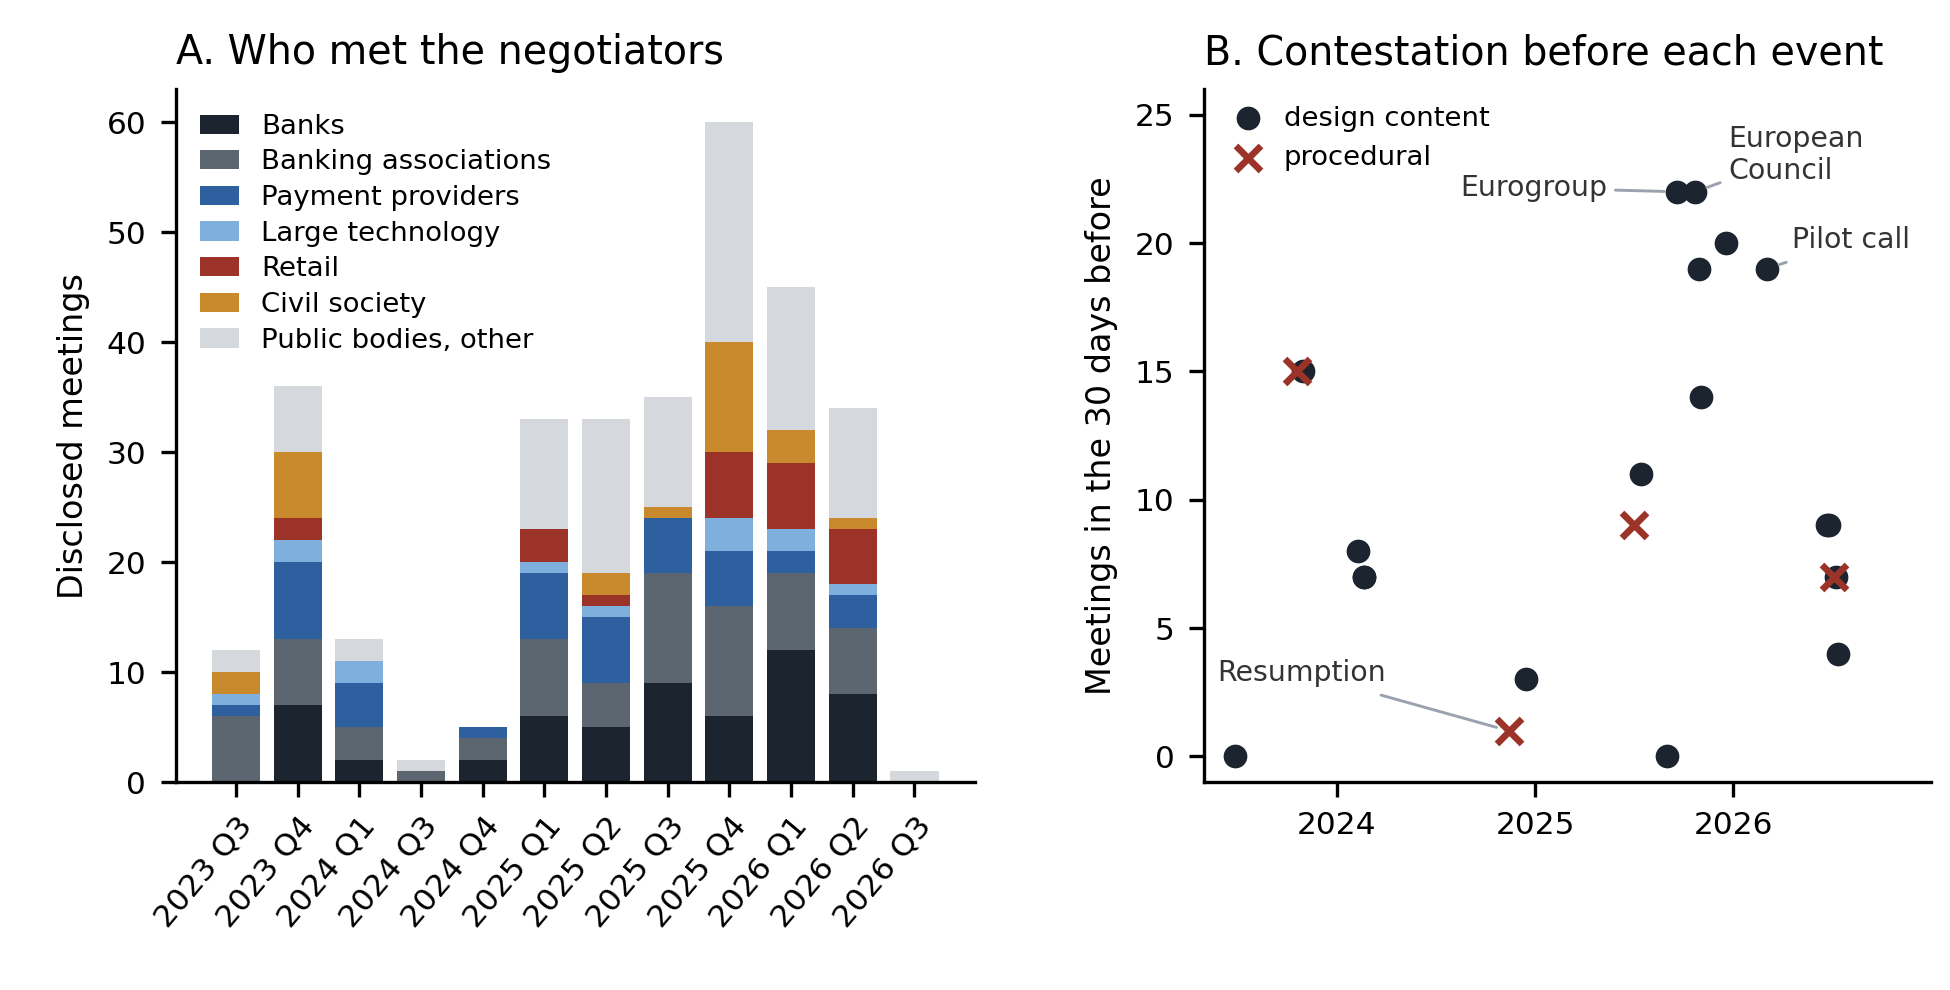
\includegraphics[width=\textwidth]{figures/fig_lobby.png}
\caption{The negotiation record for the digital euro file, 2023--2026}\label{fig:lobby}
\par\vspace{2pt}\begin{minipage}{\textwidth}\footnotesize\textit{Notes:} All 309 meetings disclosed on procedure file 2023/0212(COD) by rapporteurs, shadow rapporteurs and the committee chair, July 2023 to July 2026. Categories assigned by the author; public bodies are mostly central banks, finance ministries and permanent representations. Panel B counts meetings in the 30 calendar days before each coded event.\end{minipage}
\end{figure}

\paragraph{Who bargained.} Figure~\ref{fig:lobby}, panel A, shows the composition by quarter. Banks and banking associations account for 119 of the 309 meetings, payment providers and schemes for 40, retailers for 23, consumer and civil society organisations for 25, and large technology firms for 13. The residual category, 89 meetings, consists mostly of central banks, finance ministries and permanent representations, which we exclude from any measure of private interest.

The most frequent single counterparties are Deutsche Bank with twelve meetings, the French banking federation with ten, Amazon and the European consumer organisation with eight each, and Banco Santander and the European retail association with seven each. The presence of card networks, European payment schemes, retailers and device manufacturers alongside banks is the first piece of evidence that the incidence of this file is not confined to the deposit channel, and it is evidence that does not come from prices.

\paragraph{When they bargained.} The time profile tracks the legislative calendar rather than the news cycle: 48 meetings in 2023 around the Commission proposal, only 20 in 2024 when the file lay dormant between parliamentary terms, 161 in 2025 as the Council and the new rapporteur converged on positions, and 80 in the first seven months of 2026 up to the plenary mandate.

\paragraph{How we use it.} Panel B plots the number of meetings in the thirty days before each coded event, separating events with design content from procedural ones. Two features are relevant for the empirical design.

First, the peaks fall where the model says the stakes are: 22 meetings before the Eurogroup agreement on the ceiling mechanism of September 2025, of which 14 were held with banks or banking associations, and 19 before the ECB's call for pilot participants in March 2026, of which 13 were with the banking side.

Second, the procedural event of November 2024, the formal resumption of business after the parliamentary term, is preceded by a single meeting, against a mean of 11 before events with design content. This matters because it validates our falsification test from outside the price data. We coded that event as procedural from its content; the people who had money at stake behaved as if it were.

\paragraph{What we do not claim.} The record is used descriptively and as a measure of how contested an event was. We do not use it to determine the coded direction of any event, and we do not treat it as exogenous: firms lobby because they expect to be affected, so lobbying intensity and exposure are jointly determined. Using intensity as an instrument would be indefensible, and we do not. Publication is also mandatory only for members in a reporting capacity, so the record is a lower bound on contact rather than a census of influence.

\section{Power}\label{sec:power}

Event studies with a handful of events and a few dozen firms can be badly underpowered, and the discipline of saying so before estimation is part of the design. We simulate the second stage using the actual structure of the data: the coded direction of each event by group, the planned firm universe and the number of firms in each group. Only the noise in abnormal returns and the distribution of exposure are assumed.

Table~\ref{tab:power} reports the results. With 44 firms in the three treated groups and the 22 pre-specified estimation dates, of which ten carry a non-zero direction for banks and eight for providers, and with a standard deviation of daily abnormal returns of 1.5\%, the design detects an effect of 0.75 percentage points per unit of the exposure-direction interaction with probability 0.86. At the empirical standard deviation of 1.6\% the probability is 0.82. Under the more conservative assumption of 2.5\%, power of 0.86 is reached at 1.25 percentage points. Simulated size lies between 0.05 and 0.06. We first ran the simulation before estimation, on the 19 events coded at that time, and reached the same conclusion. The simulation draws noise independently across firms. The data show that deposit-funded banks also share shocks on a given day (Section~\ref{sec:continuous}): with such shocks the standard error of the pooled estimate is about 0.14 percentage points per standard deviation of exposure rather than 0.06, so that an effect needs to be about 0.4 to be detected with probability 0.8. That is still well below the more than one percentage point documented for 2020 and 2021.

\begin{table}[t]\centering\small
\begin{threeparttable}
\caption{Power of the second stage}\label{tab:power}
\begin{tabular}{lcccccc}
\toprule
& \multicolumn{6}{c}{Effect $\theta$ in percentage points per unit of interaction} \\
\cmidrule(lr){2-7}
Noise in abnormal returns & 0 & 0.50 & 0.75 & 1.00 & 1.25 & 1.75 \\
\midrule
$\sigma_{\text{CAR}} = 1.5\%$ & 0.06 & 0.56 & 0.86 & 0.98 & 1.00 & 1.00 \\
$\sigma_{\text{CAR}} = 1.6\%$ (empirical) & 0.05 & 0.50 & 0.82 & 0.97 & 1.00 & 1.00 \\
$\sigma_{\text{CAR}} = 2.5\%$ & 0.06 & 0.25 & 0.46 & 0.71 & 0.86 & 0.99 \\
\bottomrule
\end{tabular}
\begin{tablenotes}\footnotesize
\item \textit{Notes:} Rejection rate of a two-sided test at the 5\% level with leave-one-firm-out jackknife $t$-statistics, 2,000 replications per cell. The simulation uses the coded direction of each of the 22 pre-specified estimation dates by group and the planned firm universe (44 firms in the bank, provider and gatekeeper groups); it uses no price data. The row at 1.6\% uses the empirical standard deviation of one-day abnormal returns. Exposure is drawn uniformly on $[0.2, 0.8]$, so an interquartile move in exposure is about 0.3 units and the implied effect on abnormal returns is roughly $0.3\,\theta$. The column at $\theta=0$ reports size.
\end{tablenotes}
\end{threeparttable}
\end{table}

\paragraph{Is this enough?} The natural benchmark is the published estimate for this market. \citet{burlon2024} report that a one standard deviation difference in the deposit ratio, 18 percentage points, is associated with more than one percentage point of abnormal return per event. In the units of our interaction that corresponds to roughly 5.5 percentage points, more than four times our minimum detectable effect even under the conservative noise assumption. The design is therefore well powered against effects of the size already documented in this market, and would detect effects several times smaller. It is not powered against effects an order of magnitude smaller than the published benchmark, and we report bounded nulls as such rather than as evidence of no effect.

\section{Results}\label{sec:results}

We first report the group-level specification, fixed in advance for the case in which bank-level deposit data were not available. In that specification exposure is an indicator for membership of the treated group, which is the binary special case of equation~\eqref{eq:stage2}. The continuous specification with deposit shares is the pre-specified main test and uses variation within the bank group; Section~\ref{sec:continuous} reports it. The event coding and the firm universe were hash-frozen before any return was computed.

\subsection{Sample}

Price data were obtained for 51 of 54 series. Three failed to download: Bank of Cyprus, Fiserv and the STOXX Europe banks index. Alpha Services is available only from July 2025, after a change of listing, and drops out of earlier events for want of an estimation window. The estimation sample has 49 firms, 22 events and 1,042 firm-event observations in the one-day window. Euro area firms are benchmarked against the European three-factor model as pre-specified; firms listed in the United States are benchmarked against a market model on the S\&P~500, a choice logged before any abnormal return was computed, because European factors are not a meaningful benchmark for US equities.

\subsection{Main estimates}

\begin{table}[t]\centering\small
\begin{threeparttable}
\caption{Effect of coded design direction on abnormal returns, group-level specification}\label{tab:main}
\begin{tabular}{lcccc}
\toprule
& \multicolumn{2}{c}{One-day window} & \multicolumn{2}{c}{Two-day window} \\
\cmidrule(lr){2-3}\cmidrule(lr){4-5}
& Estimate & $t$ & Estimate & $t$ \\
\midrule
Pooled across groups & 0.055 & 0.37 & 0.093 & 0.47 \\[2pt]
Banks & 0.101 & 0.62 & 0.186 & 0.82 \\
Payment providers & $-0.147$ & $-0.36$ & $-0.287$ & $-0.94$ \\
Device gatekeepers and large technology & 0.867 & 1.68 & 1.400 & 1.60 \\
\midrule
Firms / events / observations & \multicolumn{2}{c}{49 / 22 / 1,042} & \multicolumn{2}{c}{49 / 22 / 1,032} \\
Placebo-date $p$-value, banks & \multicolumn{2}{c}{0.62} & & \\
\bottomrule
\end{tabular}
\begin{tablenotes}\footnotesize
\item \textit{Notes:} Estimates are in percentage points of abnormal return per unit of the coded design direction, which takes the values $-1$, $0$ and $+1$; under the hypothesis each coefficient is positive. Exposure is an indicator for membership of the treated group; non-euro banks are the reference group with direction zero on every event. All specifications include firm and event fixed effects. $t$-statistics use leave-one-firm-out jackknife standard errors. The placebo-date $p$-value compares the bank coefficient from a regression with the bank term alone (0.118) with its distribution when the actual coded direction vector is moved to 500 sets of random non-event trading days.
\end{tablenotes}
\end{threeparttable}
\end{table}

Table~\ref{tab:main} reports the estimates. None is statistically distinguishable from zero at conventional levels.

\textbf{Banks.} The bank coefficient is 0.10 percentage points per unit of coded direction in the one-day window and 0.18 in the two-day window. It has the predicted sign. It is not distinguishable from random trading days: moving the actual direction vector to 500 sets of non-event days produces a distribution with a 95\% band from $-0.50$ to $0.54$ percentage points, and the actual coefficient sits well inside it, with a placebo $p$-value of 0.62 (Figure~\ref{fig:bank}, panel B). The placebo exercise moves only the bank direction vector, so it uses the regression with the bank term alone, whose coefficient is 0.118 rather than the 0.101 of the full specification with all group terms; the two differ only in whether the provider and gatekeeper terms are included. The placebo band gives the most useful statement of what the design can exclude: an average differential response of euro area banks larger than about half a percentage point per unit of coded content.

\textbf{Payment providers.} There is no consistent pattern. The one-day and two-day coefficients are both small and negative, the opposite of the prediction, and neither is distinguishable from zero. The Council position of December 2025 combines a fee cap with mandated device access, whose net effect on providers the model does not sign; recoding its provider direction to zero gives $-0.38$ ($t = -1.16$), again not distinguishable from zero. The group combines international card networks, euro area acquirers and a digital wallet, and it contains two firms that suffered very large idiosyncratic price falls during the sample for reasons unrelated to the file. We do not read the two-day estimate as evidence against the fee channel; we read the group as too heterogeneous for the binary specification to be informative.

\textbf{Device gatekeepers.} The coefficient is the largest and has the predicted sign, but it cannot bear weight. The group has four firms, and only one event carries a non-zero direction for it, the Council position of 19 December 2025, which contained the device-access provision. Dropping that single event sets the coefficient to zero. This is one observation per firm, and we report it as such.

\subsection{Event by event}

\begin{figure}[t]\centering
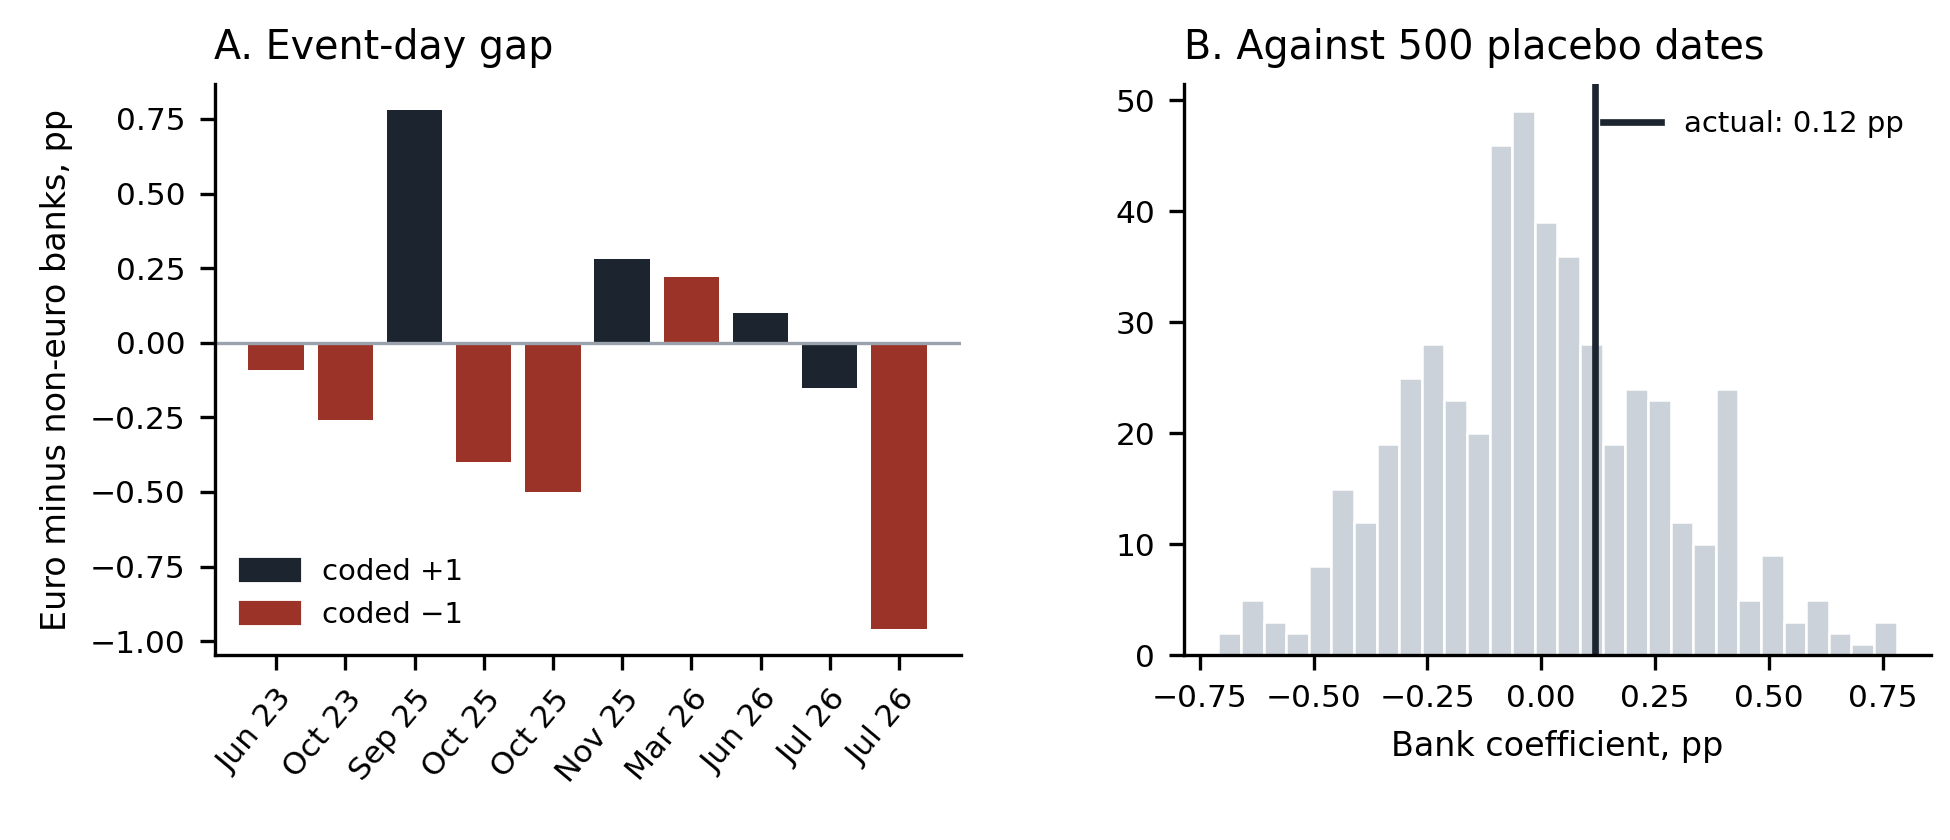
\includegraphics[width=\textwidth]{figures/fig_results_bank.png}
\caption{Banks: event-day abnormal return gap and placebo distribution}\label{fig:bank}
\par\vspace{2pt}\begin{minipage}{\textwidth}\footnotesize\textit{Notes:} Panel A: for the ten events with a non-zero coded direction for banks, the mean one-day abnormal return of 29 euro area banks minus that of 7 non-euro banks. Panel B: the bank coefficient from a regression with the bank term alone (0.118; firm and event fixed effects) against its distribution when the coded direction vector is moved to 500 sets of random non-event trading days. The full specification with all group terms gives 0.101.\end{minipage}
\end{figure}

Figure~\ref{fig:bank}, panel A, shows what lies behind the bank coefficient. For each of the ten events with a non-zero coded direction for banks, it plots the mean one-day abnormal return of euro area banks minus that of non-euro banks. The gap has the predicted sign in eight of the ten events. This observation was not part of the pre-specified analysis, and we report it as exploratory: a one-sided sign test gives $p \approx 0.055$, which is suggestive and no more. The regression coefficient is smaller than the average signed gap because the firm fixed effects absorb the fact that euro area banks earned positive abnormal returns throughout the 2023 to 2026 rally, including on days without design content.

\subsection{A falsification test we discarded, and why}

The analysis plan specified a test in which non-euro banks are assigned the same coded direction as euro area banks. In the group-level specification that test is not identified: the two regressors sum to a function of the event alone and are absorbed by the event fixed effects, so only their difference is estimable, and that difference is the main estimate itself. We computed it before recognising this, obtained coefficients that are artefacts of the collinearity, and discarded them. We replaced the test with the placebo-date randomisation, which is valid in the binary design. We report the episode because the plan promised the original test.

\subsection{What these results do and do not say}

They say that, measured at the level of the treated group, the legislative design content of the digital euro did not move the relative valuations of euro area banks, payment providers or device gatekeepers by more than about half a percentage point per event. They do not speak to the channel within banks that the model identifies, namely that banks with a larger substitutable deposit base should respond more. That test requires bank-level deposit composition and is the pre-specified main specification. It is also the more powerful one: the binary specification uses only the difference between euro area and non-euro banks, and discards the variation in exposure across 29 euro area banks.

\subsection{Continuous exposure: the main specification}\label{sec:continuous}

The pre-specified test interacts the coded direction with each euro area bank's deposit exposure, measured on 31 March 2023, the last reporting date before the Commission proposal, from the EBA transparency exercise. The primary measure is deposits of households and non-financial corporations over total liabilities, as in \citet{burlon2024}. The secondary measure, derived from Proposition~\ref{prop:conc}, uses only overnight deposits of the same sectors, since these are the balances a holding limit directly captures. Both measures and the specification were fixed and hash-frozen before estimation. Across the 29 euro area banks the deposit share averages 59\% with a standard deviation of 14 percentage points, ranging from 32\% at Mediobanca and Société Générale to 87\% at Banco Comercial Português; the two measures correlate at 0.87. Measures are standardised within euro area banks.

\begin{table}[t]\centering\small
\begin{threeparttable}
\caption{Deposit exposure and abnormal returns: main specification}\label{tab:cont}
\begin{tabular}{lcccc}
\toprule
& Estimate & Std.\ error & $t$ & Permutation $p$ \\
\midrule
\multicolumn{5}{l}{\textit{Preferred dating: draft report on 31 October 2025}} \\
Deposit share, one day & $-0.013$ & 0.084 & $-0.15$ & 0.89 \\
Deposit share, two days & 0.076 & 0.097 & 0.78 & 0.43 \\[3pt]
\multicolumn{5}{l}{\textit{Pre-specified dating, one-day window}} \\
Deposit share (pre-specified main) & 0.051 & 0.056 & 0.92 & 0.45 \\
Overnight deposit share & 0.060 & 0.054 & 1.12 & 0.35 \\
Deposit share, excluding Crédit Agricole & 0.053 & & 0.94 & \\[3pt]
\multicolumn{5}{l}{\textit{Pre-specified dating, two-day window}} \\
Deposit share & 0.131 & 0.092 & 1.42 & 0.15 \\
Overnight deposit share & 0.075 & 0.084 & 0.90 & 0.41 \\
\bottomrule
\end{tabular}
\begin{tablenotes}\footnotesize
\item \textit{Notes:} Estimates are percentage points of abnormal return per standard deviation of exposure per unit of coded design direction; under the hypothesis they are positive. Exposure is measured on 31 March 2023 and standardised across the 29 euro area banks. The regression also contains the group-level direction terms of Table~\ref{tab:main} and firm and event fixed effects. Standard errors are leave-one-firm-out jackknife; standard errors that also allow for shocks common to all banks on an event day are in the text and in Table~\ref{tab:referee}. The permutation $p$-value reassigns exposure across euro area banks, 9,999 draws. In the preferred dating the draft report is dated by the first trading day after its content was reported (Section~\ref{sec:inst}). Crédit Agricole is excluded in one row because the supervisory data refer to the consolidated group while the listed entity is Crédit Agricole SA.
\end{tablenotes}
\end{threeparttable}
\end{table}

Table~\ref{tab:cont} reports the results. None of the coefficients is statistically distinguishable from zero. In the preferred specification the relative gain of a bank one standard deviation more exposed to deposit substitution, on an event coded as limiting the digital euro, is $-0.013$ percentage points, with a permutation $p$-value of 0.89; over two days it is 0.08 ($p = 0.43$). With the pre-specified dating every coefficient has the predicted sign: 0.05 in the one-day window ($p = 0.45$), 0.06 with the overnight measure, our mechanism-motivated proxy for the substitutable deposit base, and 0.13 over two days ($p = 0.15$). Excluding the bank whose supervisory and listed perimeters differ changes nothing.

\paragraph{Shocks common to an event day.} The leave-one-firm-out jackknife and the exposure permutation treat the firm as the unit of independent variation. On any trading day, however, deposit-funded banks can move together for reasons unrelated to the event, and with 22 events such day-level shocks need not average out. Two procedures allow for them. Dropping one event at a time gives a jackknife standard error over events of 0.139 for the preferred estimate and 0.144 for the pre-specified one, against 0.084 and 0.056 over firms. Assigning the 22 coded direction vectors in random order to 22 non-event trading days, 2,000 times, gives a placebo distribution with a standard deviation of 0.115 (0.112 for the pre-specified dating) and a 95\% band from $-0.22$ to $0.22$; the placebo-date $p$-value is 0.91 for the preferred estimate and 0.65 for the pre-specified one. Day-level shocks are therefore the larger source of uncertainty in this design, and we use the event-level standard errors for the bounds below.

\paragraph{What the exposure permutation assumes.} Deposit funding is not randomly assigned across banks; it varies with country, business model and size. Permuting exposure across euro area banks is therefore not design-based randomisation inference. It is valid under exchangeability of the exposure labels conditional on the fixed effects: if exposure has no effect on event-day returns, reassigning it across banks leaves the distribution of the statistic unchanged. Two variants make the assumption weaker. Permuting only within country, so that a German bank's exposure is only ever assigned to another German bank, gives $p = 0.43$ across ten country blocks. Residualising exposure on country, so that only within-country differences in deposit funding identify the coefficient, gives $0.011$ percentage points per standard deviation ($t = 0.23$). Neither changes the conclusion.

\paragraph{Robustness of the main estimate.} Several checks bear on the reading of Table~\ref{tab:cont}. The pre-specified variations of window, estimation sample, factor model and event dating in Table~\ref{tab:robust} leave the estimate between $-0.014$ and $0.061$; a conventional per-event pre-event estimation window gives $0.099$ ($t=1.83$), and $0.043$ ($t = 0.57$) with the draft report dated by its first press report. Dropping each event in turn moves the pre-specified coefficient between $-0.005$ and $0.153$ percentage points; the upper value arises when the ECB's call for pilot participants of 5 March 2026 is removed, an event on which the most deposit-funded banks outperformed the least deposit-funded ones against the coded direction. A null-imposed wild cluster bootstrap with Rademacher weights on firms gives $p = 0.33$. Restricting the sample to the five events coded as highly surprising before any price was seen gives $0.014$ ($t = 0.11$). The last check matters for interpretation: if the null reflected anticipation of scheduled steps, the unscheduled and contested events should show the effect, and they do not. The pre-specified falsification test F1 also holds: adding the interaction of exposure with an indicator for the four procedural dates to the main specification gives a slope of 0.04 percentage points per standard deviation on those dates ($t = 0.55$, permutation $p = 0.73$) and leaves the pre-specified estimate at 0.05. Two further checks concern the first stage and the exposure measure. A euro-denominated market model in excess returns, with loadings estimated separately for each event on days strictly before it, gives 0.026 ($t = 0.37$) in the preferred dating and 0.076 ($t = 1.61$) in the pre-specified one. And the deposit share of 31 December 2019, from the transparency exercise published in 2020 and therefore public at every event, gives $-0.002$ ($t = -0.02$) and 0.051 ($t = 0.89$); the 2023 measure refers to a date before the proposal but was published only in December 2023.


\paragraph{Event by event.} Figure~\ref{fig:slopes_all} in Section~\ref{sec:early} decomposes the estimate. For each bank-relevant event it shows the cross-sectional slope of abnormal returns on deposit exposure, signed so that positive values agree with the prediction. Five of the ten slopes are positive, and three of them are individually around 0.4 to 0.5 percentage points per standard deviation: the ECB opinion of October 2023, the rapporteur's paper of September 2025 and the European Council of October 2025. The draft report, on 31 October 2025, has a slope of $-0.18$; at its document date of 3 November 2025 it was 0.42. The events of 2026 are zero or negative, and the pilot call of March 2026 is strongly negative. On ordinary trading days of 2023 to 2026 single-day slopes have a standard deviation of 0.34, so that apart from the pilot call no individual slope stands out from day-level noise. This pattern is exploratory, since the pre-specified analysis pools the events, and with ten events it can be noise. It is nonetheless informative about the size of the effects at stake. Where the slopes agree with the prediction, they are around 40\% of the magnitude reported for 2020 and 2021; nowhere do they approach it; and the events at which the legislative outcome was confirmed, in June and July 2026, show nothing.

\paragraph{Multiple testing and the provider exposure measure.} The plan specified two things for the non-bank groups that we report here in the form the data allow. First, a continuous exposure measure for payment providers, their share of revenue earned on euro area transactions. We did not assemble segment-level revenue data for these firms, so the provider coefficient is estimated with a group indicator throughout; this is a deviation from the plan and is recorded as such. Second, the three group-level predictions were to be adjusted jointly with the step-down procedure of \citet{romano2005}. Using the placebo-date resampling of Section~\ref{sec:results} to approximate the joint null distribution, the adjusted $p$-values are 0.88 for banks, 0.88 for payment providers and 0.85 for device gatekeepers, against unadjusted $p$-values from the same joint resampling of 0.65, 0.73 and 0.40. The unadjusted bank value differs from the 0.62 of Table~\ref{tab:main} because the joint resampling studentises the coefficients of the full specification with all three group terms over 300 draws, while Table~\ref{tab:main} uses the regression with the bank term alone and 500 draws.

\paragraph{What the null excludes.} With event-level standard errors, the 95\% confidence interval of the preferred estimate runs from $-0.29$ to $+0.26$ percentage points per standard deviation, and that of the pre-specified estimate from $-0.23$ to $+0.33$; with firm-level standard errors the intervals are $-0.18$ to $+0.15$ and $-0.06$ to $+0.16$. \citet{burlon2024} find that during the 2020 and 2021 announcements a one standard deviation higher deposit ratio was associated with more than one percentage point lower abnormal return per event. Allowing for the difference in the sign convention, their magnitude lies about four times above the upper end of the event-level interval of the preferred estimate and three times above that of the pre-specified one. The legislative design events of 2023 to 2026 therefore moved bank valuations, per unit of deposit exposure, by at most a quarter to a third of what the ECB's early announcements did.

\paragraph{Was the design priced earlier?} A natural reading of the null is that the market learned the essential design before the legislators took up the file. \citet{burlon2024} document that the trend in bank valuations reversed after the Executive Board first mentioned a holding limit of about EUR 3,000 in February 2021. If the cap was priced then, its later legislative refinement carried little news. We test this directly in Section~\ref{sec:early}.

\subsection{Extending the sample to 2020 and 2021}\label{sec:early}

We extend the price data back to June 2019 and code six events of 2020 and 2021 from the ECB's own record, verified at the relevant press releases: the Eurosystem report on a digital euro of 2 October 2020, the launch and the close of the public consultation, the Executive Board's statement of 10 February 2021 that a holding limit of around EUR 3,000 was under consideration, the publication of the consultation results, and the launch of the investigation phase on 14 July 2021. Three carry a non-zero direction for banks: the report and the investigation phase, which advance the project ($-1$), and the holding-limit statement, which is the first quantitative signal of a cap ($+1$). The consultation steps carry no design content. As before, the coding was fixed and hash-frozen before any return from the new price file was computed, and the test was specified in advance: the same regression as the main specification, on the early events, with the prediction that the early coefficient is large and positive.

\begin{figure}[t]\centering
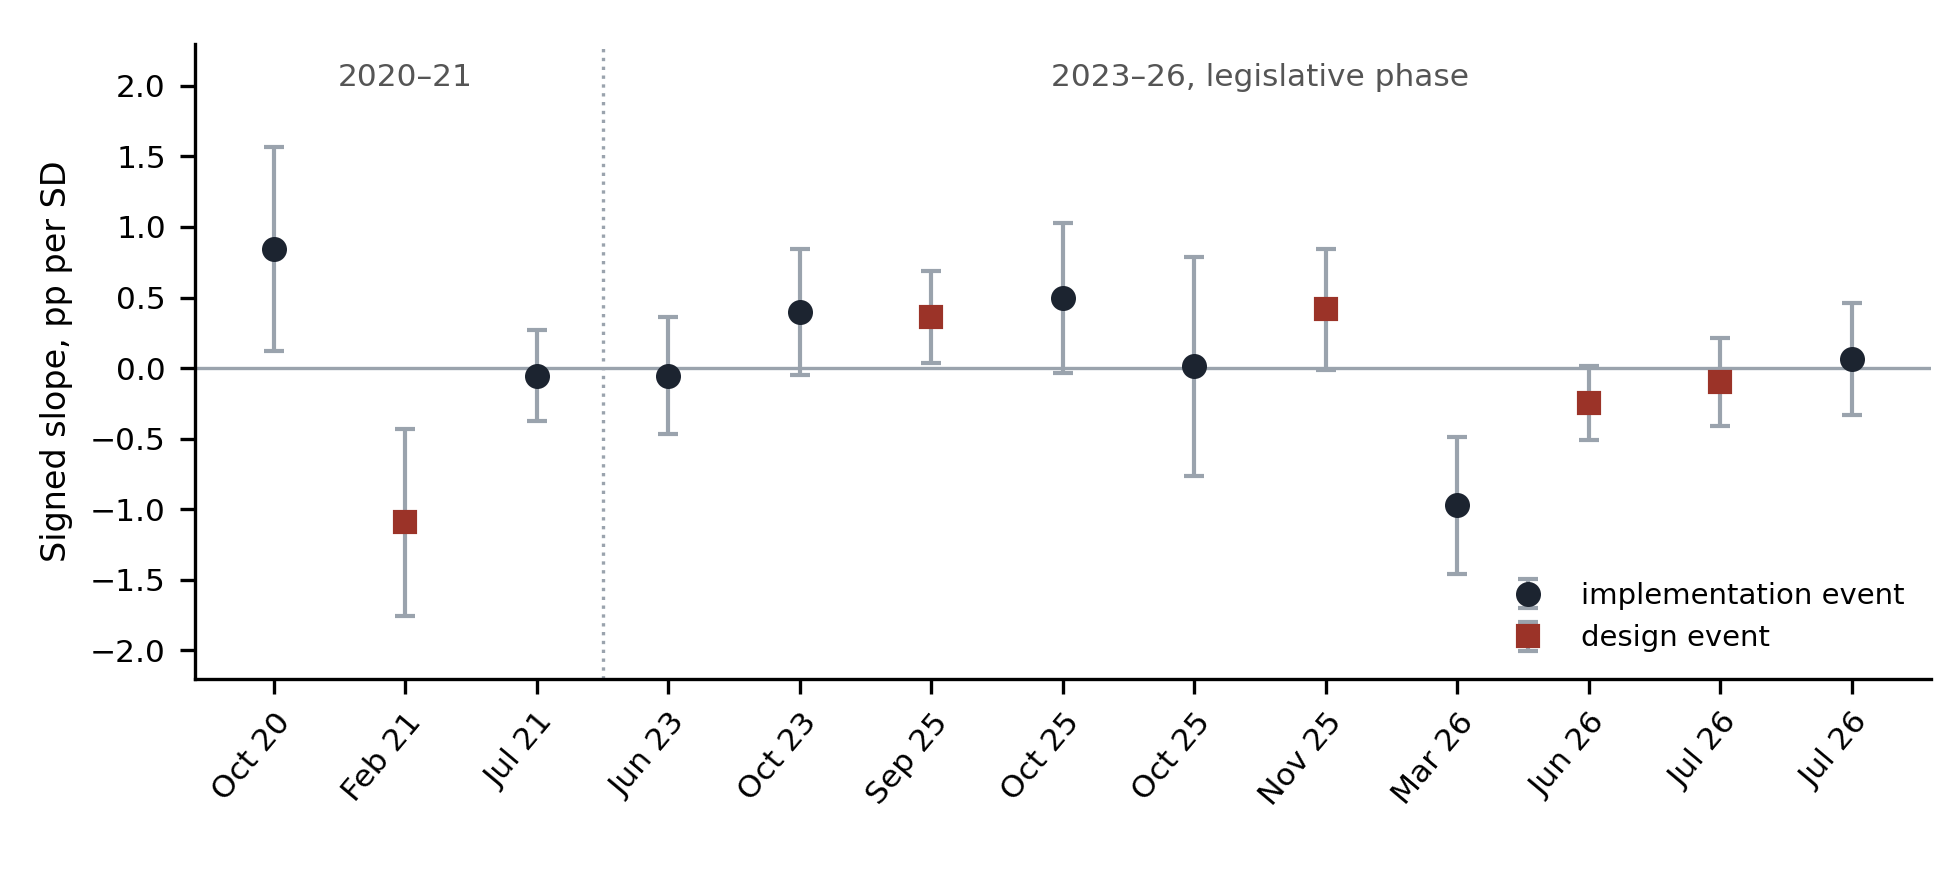
\includegraphics[width=\textwidth]{figures/fig_event_slopes_all.png}
\caption{Deposit exposure and abnormal returns, event by event, 2020 to 2026}\label{fig:slopes_all}
\par\vspace{2pt}\begin{minipage}{\textwidth}\footnotesize\textit{Notes:} For each event with a non-zero coded direction for banks, the cross-sectional slope of the one-day abnormal return of euro area banks on their standardised deposit share, multiplied by the coded direction so that positive values agree with the prediction. Bars are 95\% intervals. Deposit shares are measured on 31 December 2019 for the 2020 to 2021 events and on 31 March 2023 for the legislative events. The draft report is shown on 31 October 2025, the first trading day after its content was reported (preferred dating); at its document date of 3 November 2025 the signed slope is 0.42.\end{minipage}
\end{figure}

\paragraph{The pre-specified test does not support the reading.} Exposure for the early events is measured on 31 December 2019, from the EBA transparency exercise of spring 2020, so that it is predetermined; its correlation with the 2023 measure across the 29 euro area banks is 0.97. The early coefficient is $-0.27$ percentage points per standard deviation of deposit exposure, with $t = -1.47$ and a permutation $p$-value of 0.14. It has the wrong sign and is not distinguishable from zero. The claim that the cap was priced in 2021 is not supported by our data.

\paragraph{But the design can see a Burlon-sized effect when there is one.} Figure~\ref{fig:slopes_all} shows why the pooled coefficient is uninformative about the early period. On the day the Eurosystem published its report, the most deposit-funded banks underperformed the least deposit-funded ones by 0.85 percentage points per standard deviation of exposure (standard error 0.37), with the predicted sign and a magnitude close to the one reported by \citet{burlon2024} for the same period. The cross-sectional standard error understates the noise of a single day. Against the slopes of the 529 trading days of July 2019 to December 2021 without digital euro news, whose standard deviation is 0.45, the report-day slope is larger in absolute value than 94\% of them (two-sided $p = 0.06$). On the day the holding limit was first floated, the slope was $-1.09$ (standard error 0.34), outside the central 95\% of daily slopes: the most deposit-funded banks again underperformed, which is the opposite of what a favourable design signal predicts. The launch of the investigation phase shows nothing.

Two conclusions follow. First, the report day is a positive control. With the same firms, the same exposure measure, the same factor model and the same estimator, the design finds a slope close to the size documented in the literature when the news is about whether a digital euro will exist, at the edge of what day-level noise produces. A single day is weak evidence; pooled over 22 events, however, an effect of that size would stand out clearly, since the event-level standard error of the pooled estimate is about 0.14. The null for the legislative phase is therefore not a failure of the design to see effects of the documented size. Second, neither the first cap signal in 2021 nor the legislative design events of 2023 to 2026 moved deposit-funded banks in the direction the design channel predicts. The pattern is consistent with the market having reacted to news about the existence of the project, early, rather than to news about its design; with a single early event of this kind we state it as a pattern, not as an established fact.

Three remarks on robustness. The baseline first stage estimates factor loadings on a common window that lies after these events; estimating them instead on the 250 trading days strictly before each event gives a report-day slope of 0.77 (standard error 0.36) with the European three-factor model and 0.82 (0.37) with a euro-denominated market model in excess returns, and a holding-limit-day slope of $-1.09$ in both, so the positive control does not depend on post-event information. Using the 2023 exposure measure for the early events instead gives a report-day slope of 1.06, a holding-limit-day slope of $-1.21$ and a pooled coefficient of $-0.24$, so the choice of measurement date does not matter. Finally, single-day slopes can be driven by news unrelated to the digital euro; the report-day estimate is an individual event, not a replicated pattern, and we present it as a demonstration that the design has power rather than as a finding in its own right.

\subsection{Additional analyses}\label{sec:referee}

The analyses in this section were added after a review of the first complete draft. They were not part of the pre-specified plan and are reported as such, alongside the pre-specified estimate rather than in place of it.

\begin{table}[t]\centering\small
\begin{threeparttable}
\caption{Additional analyses of the deposit-exposure specification}\label{tab:referee}
\begin{tabular}{lcccc}
\toprule
& Estimate & $t$ & Permutation $p$ & Events \\
\midrule
Pre-specified specification & 0.051 & 0.92 & 0.45 & 22 \\
Without events coded with ex-post information & 0.051 & 0.93 & 0.45 & 20 \\[3pt]
\multicolumn{5}{l}{\textit{Separating the kinds of event}} \\
\quad Design-parameter events & $-0.004$ & $-0.04$ & 0.97 & 4 \\
\quad Implementation events & 0.096 & 0.95 & & 6 \\
\quad Design-parameter events, draft report dated 31 October & $-0.148$ & $-1.18$ & 0.35 & 4 \\[3pt]
\multicolumn{5}{l}{\textit{Timing}} \\
\quad Draft report dated by first press report, 31 October 2025 & $-0.013$ & $-0.15$ & 0.89 & 22 \\
\quad Timestamp-aligned, all events & 0.043 & 0.48 & 0.66 & 22 \\
\quad Timestamp-aligned, excluding confounded days & 0.029 & 0.36 & & 20 \\
\quad Timestamp-aligned, design-parameter events only & $-0.065$ & $-0.35$ & 0.71 & 4 \\
\quad Earlier timestamp alignment, all events & 0.161 & 1.82 & 0.075 & 22 \\
\quad European Council event moved to next trading day & 0.011 & 0.20 & & 22 \\
\quad Excluding the two days with major same-day news & $-0.005$ & $-0.09$ & & 20 \\[3pt]
\multicolumn{5}{l}{\textit{Inference allowing for event-day shocks}} \\
\quad Preferred dating, event jackknife; placebo dates & $-0.013$ & $-0.09$ & 0.91 & 22 \\
\quad Pre-specified dating, event jackknife; placebo dates & 0.051 & 0.36 & 0.65 & 22 \\[3pt]
\multicolumn{5}{l}{\textit{Placebo: the same exposure slope for non-euro banks}} \\
\quad Euro area banks & 0.051 & & & \\
\quad Non-euro banks (four) & 0.182 & 1.10 & & \\
\quad Difference, euro minus non-euro & $-0.131$ & & & \\
\bottomrule
\end{tabular}
\begin{tablenotes}\footnotesize
\item \textit{Notes:} Percentage points of one-day abnormal return per standard deviation of the deposit share per unit of coded direction. Non-euro banks are assigned the coded bank direction of each event and their deposit share standardised on the euro area scale; the four are Danske Bank, Swedbank, Handelsbanken and DNB; the three non-euro banks without EBA data are excluded from this test. The pre-specified specification is that of Table~\ref{tab:cont}. Standard errors are leave-one-firm-out jackknife; permutation reassigns exposure across euro area banks, 9,999 draws. Timestamp-aligned rows use the documented release times of Section~\ref{sec:flow}, with the draft report on 31 October 2025 and the ECB release of 30 October 2025 in a one-day window; the null-imposed wild cluster bootstrap $p$-value is 0.61. The earlier alignment treated both releases as undocumented and used two-day windows for them; its wild bootstrap $p$-value is 0.053. In the rows allowing for event-day shocks, $t$ uses the leave-one-event-out jackknife standard error (0.139 and 0.144) and the $p$-value comes from 2,000 draws of placebo dates, which assign the coded direction vectors to random non-event trading days. ``Events'' counts estimation dates, or for the split, dates with a non-zero bank direction of each kind.
\end{tablenotes}
\end{threeparttable}
\end{table}

\paragraph{Currency and a correction to the window rule.} The pre-specified first stage regresses local-currency returns on the European Fama--French factors, which are computed in US dollars. Two alternatives address this. Replacing only the market factor by the euro-denominated STOXX Europe 600 return, while keeping the dollar-based size and value factors, gives 0.042 in the one-day window, 0.115 in the two-day window, 0.030 in the release-time-aligned specification and $-0.003$ on design events. A fully euro-denominated market model in excess returns, with the ECB deposit facility rate as the risk-free rate, gives 0.054 in the one-day window ($t = 0.95$) and $-0.001$ on design events; in the release-time-aligned specification it gives 0.047 (standard error 0.085, 95\% confidence interval $-0.12$ to 0.21), with a permutation $p$-value of 0.61 and a wild cluster bootstrap $p$-value of 0.58 (Table~\ref{tab:robust}). With the draft report dated by its first press report, the one-day estimates are $-0.021$ and $-0.010$. The results do not depend on the benchmark. In the earlier timestamp alignment of Section~\ref{sec:flow} the benchmark did matter: the euro-denominated market model gave 0.167, with a permutation $p$-value of 0.050 and a wild bootstrap $p$-value of 0.024. That was the strongest evidence for a small effect in the paper, and it does not survive the correct dating of the draft report under any benchmark. In the course of these checks we also found that two-day windows had been summed over whichever days had a return rather than requiring both; the corrected rule reduces the two-day sample from 1,069 to 1,032 observations, leaves the bank estimates essentially unchanged, and reduces the two-day payment-provider coefficient from $-0.51$ to $-0.29$. All results reported here use the corrected rule.

\paragraph{No look-ahead.} Excluding the two 2024 events whose pre-specified coding relied on the later fate of the draft leaves the estimate unchanged at 0.051 percentage points, because both carried a zero direction and entered only through the fixed effects.

\paragraph{Design parameters alone.} Restricting the treatment to events that fixed or signalled a design parameter gives, in the pre-specified dating, an estimate of $-0.004$ percentage points per standard deviation, with a permutation $p$-value of 0.97, and $-0.15$ in the preferred dating (see below). In the pre-specified dating the small positive coefficient of the pooled specification comes entirely from implementation events, and even there it is not distinguishable from zero. This is the sharpest answer to the question in the title, and it should be read with its precision. Four design-parameter events carry a bank direction; the standard error is 0.11 and the 95\% confidence interval runs from $-0.22$ to $0.21$ percentage points per standard deviation. We therefore detect no price effect of the design parameters. With firm-level standard errors the interval excludes effects a fifth the size documented for 2020 and 2021, but with four events this understates the uncertainty, and it does not exclude small effects. Three further statements make the precision explicit. First, simulating the design-only coefficient on the actual structure of the data, four design events, 29 euro area banks with their observed exposure and the empirical dispersion of abnormal returns, the test has power of 0.54 against an effect of 0.4 percentage points per standard deviation, 0.77 against 0.5 and 0.90 against 0.6, with simulated size of 0.07. The simulation draws noise independently across firms; with day-level shocks of the size estimated in Section~\ref{sec:continuous}, power is lower still. The design-only test is therefore informative against effects of about half the documented magnitude or more, and not against smaller ones. Second, the null does not come from a single event. The four event-level slopes, signed so that positive values agree with the prediction, are 0.36 (the rapporteur's paper), 0.42 (the draft report at its document date), $-0.24$ (the committee position) and $-0.10$ (the plenary mandate): two in each direction, none large. With four events a sign test carries no information, and we do not report one as evidence. Third, the dating of the draft report matters for the sign but not for the conclusion. On 31 October 2025, the first trading day after its content was reported, the slope is $-0.18$, and the design-only coefficient becomes $-0.15$ (standard error 0.13, permutation $p = 0.35$), with the wrong sign; in the timestamp-aligned specification with documented release times it is $-0.06$ (standard error 0.19). None of these is distinguishable from zero.

\paragraph{Placebo on non-euro banks.} If the exposure slope reflected the digital euro, it should be absent for banks outside the euro area, which have comparable deposit structures and no exposure to the instrument. Assigning the same coded directions to the four non-euro banks with supervisory data gives a slope of 0.18 percentage points per standard deviation, larger than for euro area banks, with $t = 1.10$. The difference between euro area and non-euro banks is $-0.13$. Whatever small co-movement exists between deposit funding and returns on event days does not appear to be specific to the euro area. It is consistent with a generic factor loading on deposit-funded banks rather than a response to the digital euro, although four control banks cannot establish this. With four control banks the test is weak, but it points in the direction that reinforces the null rather than the hypothesis.


\section{Conclusion}

A central bank digital currency redistributes rents along the payments chain, and the size of that redistribution is set by its design parameters. We measured the price of those parameters over the three years in which the European co-legislators adopted and narrowed their positions on them, coding each act by its content for banks, payment providers and device gatekeepers before looking at any price, and complementing the price evidence with the complete record of who negotiated with the legislators.

The answer is that the legislative phase moved valuations little, if at all. With every event dated by the day its content became public, the relative gain of a euro area bank one standard deviation more exposed to deposit substitution, on an event that limited the digital euro, was $-0.01$ percentage points; with the pre-specified dating it was 0.05. Allowing for shocks common to all banks on an event day, the confidence intervals exclude effects about a quarter and a third the size of those documented for the ECB's announcements of 2020 and 2021. The bound survives the pre-specified robustness checks, a currency-consistent first stage with strictly pre-event loadings, exposure measured from data public before every event, the alignment of events to their documented release times and a restriction to events that were contested and unscheduled, which argues against anticipation as the explanation. Aligning all events to their documented release times gives 0.03 to 0.05 with permutation $p$-values above 0.6. An earlier alignment that gave 0.15 to 0.17, significant at the 10\% level by the wild bootstrap, did so because it attributed the market's reaction to the draft report to the ECB release of the previous day. On the events that set or signalled a design parameter, as opposed to events that only changed the probability of issuance, the estimate is $-0.15$ in the preferred dating and $-0.004$ in the pre-specified one: we detect no price effect of the design parameters. And the small positive slope that remains in the pooled pre-specified estimate appears, if anything, larger for banks outside the euro area, which is consistent with a generic factor loading on deposit-funded banks rather than a digital-euro-specific response.

For financial stability the implication is direct. The concern that motivated the holding limit was deposit flight from banks. Markets did not price a large residual flight risk into euro area bank valuations during the legislative process; any effect on the most exposed banks appears modest relative to their response to the early announcements. The market did react to digital euro news: on the day the Eurosystem report was published in October 2020, deposit-funded banks underperformed by 0.85 percentage points per standard deviation of predetermined exposure. But that was news about whether the instrument would exist. News about how it would be designed, from the first cap signal in 2021 to the legislative texts of 2023 to 2026, did not generate a consistent or statistically detectable response of deposit-funded banks in the predicted direction. The negotiation record shows that the parameters were nonetheless intensely contested, with 309 documented meetings and the banking side accounting for the largest share. Whatever the banks were bargaining over did not generate a large detectable valuation response in equity markets.

The evidence has limits that bear on how it should be read. An absent valuation response shows that investors did not expect the parameters to change bank value by much; it does not show that the parameters are without economic effect. Effects on lending, deposit pricing or liquidity management that investors regarded as immaterial to value, or that will appear only once the instrument is issued, are outside what equity prices can reveal. The deposit share is a proxy for the substitutable balance rather than a measure of it, and four design events carry a bank direction. The coding records the direction of each act, not its size in euro, so the estimates are valuation responses to decisions, not the value of one more euro of holding limit. Within these limits the bound is informative, because the same proxy and the same design find a slope of the documented size on the day the Eurosystem report appeared, and an effect of that size, pooled over the legislative events, would stand out clearly from day-level noise.

Two questions remain open. First, whether the null extends to lending and deposit pricing, which equity prices do not observe; bank-level lending data around the design events would answer it. Second, whether exact timing matters further. Documenting the release time of two events moved the aligned estimate from 0.16 to 0.04; eleven releases still lack a documented time of day, and intraday timestamps for them would settle whether the windows hide a small effect.


\clearpage
\bibliographystyle{plainnat}
\section*{Data and code availability}
All data used in this paper are public. Event documents come from EUR-Lex, the Legislative Observatory, the Council, the Eurogroup and the ECB (sources in Table~\ref{tab:allevents}); the negotiation record is transcribed from procedure file 2023/0212(COD). Bank exposure comes from the EBA EU-wide transparency exercises of 2020 and 2023, factor returns from the Kenneth French Data Library, and the deposit facility rate from the ECB Data Portal (series FM.D.U2.EUR.4F.KR.DFR.LEV). Share prices are from Yahoo Finance, whose terms govern redistribution; the package includes the scripts that retrieve them. The replication package contains the event coding, the negotiation record, the derived data, every estimation and figure script, a master script that reproduces all tables and figures, and the analysis plan with its dated SHA-256 freeze hashes: \url{https://github.com/Philip-Kroos/The-Price-of-a-Design-Parameter-Bank-Valuations-in-the-Digital-Euro-Legislative-Process}.

\begin{thebibliography}{99}
\bibitem[Andolfatto(2021)]{andolfatto2021} Andolfatto, D. (2021). Assessing the Impact of Central Bank Digital Currency on Private Banks. \emph{Economic Journal} 131(634), 525--540.
\bibitem[Auer et al.(2025)]{auer2025} Auer, S., N. Branzoli, G. Ferrero, A. Ilari, F. Palazzo and E. Rainone (2025). CBDC and the Banking System. \emph{Journal of Economics and Statistics} 245(4--5), 435--478.
\bibitem[Berg et al.(2024)]{berg2024} Berg, T., J. Keil, F. Martini and M. Puri (2024). CBDCs, Payment Firms, and Geopolitics. Discussion Paper 19367, CEPR.
\bibitem[Bertrand et al.(2014)]{bertrand2014} Bertrand, M., M. Bombardini and F. Trebbi (2014). Is It Whom You Know or What You Know? An Empirical Assessment of the Lobbying Process. \emph{American Economic Review} 104(12), 3885--3920.
\bibitem[Bidder et al.(2024)]{bidder2024} Bidder, R., T. Jackson and M. Rottner (2024). CBDC and Banks: Disintermediating Fast and Slow. Discussion Paper 15/2024, Deutsche Bundesbank.
\bibitem[Binder(1985)]{binder1985} Binder, J. J. (1985). Measuring the Effects of Regulation with Stock Price Data. \emph{RAND Journal of Economics} 16(2), 167--183.
\bibitem[Brunnermeier and Niepelt(2019)]{brunnermeier2019} Brunnermeier, M. K. and D. Niepelt (2019). On the Equivalence of Private and Public Money. \emph{Journal of Monetary Economics} 106, 27--41.
\bibitem[Burlon et al.(2024)]{burlon2024} Burlon, L., M. Muñoz and F. Smets (2024). The Optimal Quantity of CBDC in a Bank-Based Economy. \emph{American Economic Journal: Macroeconomics} 16(4), 172--217.
\bibitem[Cameron et al.(2008)]{cameron2008} Cameron, A. C., J. B. Gelbach and D. L. Miller (2008). Bootstrap-Based Improvements for Inference with Clustered Errors. \emph{Review of Economics and Statistics} 90(3), 414--427.
\bibitem[Chapman et al.(2023)]{chapman2023} Chapman, J., J. Chiu, M. Davoodalhosseini, J. H. Jiang, F. Rivadeneyra and Y. Zhu (2023). Central Bank Digital Currencies and Banking: Literature Review and New Questions. Staff Discussion Paper 2023-4, Bank of Canada.
\bibitem[Chiu et al.(2023)]{chiu2023} Chiu, J., S. M. Davoodalhosseini, J. Jiang and Y. Zhu (2023). Bank Market Power and Central Bank Digital Currency: Theory and Quantitative Assessment. \emph{Journal of Political Economy} 131(5), 1213--1248.
\bibitem[Drechsler et al.(2017)]{drechsler2017} Drechsler, I., A. Savov and P. Schnabl (2017). The Deposits Channel of Monetary Policy. \emph{Quarterly Journal of Economics} 132(4), 1819--1876.
\bibitem[European Central Bank(2025)]{ecb2025} European Central Bank (2025). Preparation Phase of a Digital Euro: Closing Report. Frankfurt am Main, October 2025.
\bibitem[Fama and French(1993)]{fama1993} Fama, E. F. and K. R. French (1993). Common Risk Factors in the Returns on Stocks and Bonds. \emph{Journal of Financial Economics} 33(1), 3--56.
\bibitem[Fern\'andez-Villaverde et al.(2021)]{fernandezvillaverde2021} Fern\'andez-Villaverde, J., D. Sanches, L. Schilling and H. Uhlig (2021). Central Bank Digital Currency: Central Banking for All? \emph{Review of Economic Dynamics} 41, 225--242.
\bibitem[Igan et al.(2012)]{igan2012} Igan, D., P. Mishra and T. Tressel (2012). A Fistful of Dollars: Lobbying and the Financial Crisis. \emph{NBER Macroeconomics Annual} 26, 195--230.
\bibitem[Keister and Sanches(2023)]{keister2023} Keister, T. and D. Sanches (2023). Should Central Banks Issue Digital Currency? \emph{Review of Economic Studies} 90(1), 404--431.
\bibitem[Kolari and Pynn\"onen(2010)]{kolari2010} Kolari, J. W. and S. Pynn\"onen (2010). Event Study Testing with Cross-Sectional Correlation of Abnormal Returns. \emph{Review of Financial Studies} 23(11), 3996--4025.
\bibitem[Kroszner and Stratmann(1998)]{kroszner1998} Kroszner, R. S. and T. Stratmann (1998). Interest-Group Competition and the Organization of Congress: Theory and Evidence from Financial Services' Political Action Committees. \emph{American Economic Review} 88(5), 1163--1187.
\bibitem[Lambert et al.(2024)]{lambert2024} Lambert, C., B. Meller, C. Pancaro, A. Pellicani, P. Radulova, O. Soons and A. van der Kraaij (2024). Digital Euro Safeguards: Protecting Financial Stability and Liquidity in the Banking Sector. Occasional Paper 346, European Central Bank.
\bibitem[MacKinlay(1997)]{mackinlay1997} MacKinlay, A. C. (1997). Event Studies in Economics and Finance. \emph{Journal of Economic Literature} 35(1), 13--39.
\bibitem[Meller and Soons(2023)]{meller2023} Meller, B. and O. Soons (2023). Know Your (Holding) Limits: CBDC, Financial Stability and Central Bank Reliance. Occasional Paper 326, European Central Bank.
\bibitem[Mu\~noz and Soons(2023)]{munoz2023} Mu\~noz, M. A. and O. Soons (2023). Public Money as a Store of Value, Heterogeneous Beliefs, and Banks: Implications of CBDC. Working Paper 2801, European Central Bank.
\bibitem[Rochet and Tirole(2003)]{rochet2003} Rochet, J.-C. and J. Tirole (2003). Platform Competition in Two-Sided Markets. \emph{Journal of the European Economic Association} 1(4), 990--1029.
\bibitem[Romano and Wolf(2005)]{romano2005} Romano, J. P. and M. Wolf (2005). Stepwise Multiple Testing as Formalized Data Snooping. \emph{Econometrica} 73(4), 1237--1282.
\bibitem[Schwert(1981)]{schwert1981} Schwert, G. W. (1981). Using Financial Data to Measure Effects of Regulation. \emph{Journal of Law and Economics} 24(1), 121--158.
\end{thebibliography}

\clearpage
\appendix
\renewcommand{\thesection}{\Alph{section}}

\section{Codebook and full event list}\label{app:codebook}

\subsection{Coding rules}
Except for the two February 2024 events documented in Table~\ref{tab:allevents}, whose text was not available, each event is assigned from the contemporaneously available text of the act alone, before any price data is loaded:
\begin{itemize}\itemsep1pt
\item \textbf{Procedural}: one if the act contains no provision bearing on any design parameter.
\item \textbf{Direction by group}, in $\{-1,0,+1\}$, separately for banks, payment providers and device gatekeepers. Positive means the act raises the rent of that group relative to the status quo ante, by the logic of Propositions~\ref{prop:quantity} to \ref{prop:access}. A blank denotes an act with no provision bearing on that group.
\item \textbf{Dose}: the quantitative parameter named in the act, where one is named.
\item \textbf{Surprise}: none, low, medium or high, from the prior public record.
\item \textbf{Justification}: the provision on which the coding rests, recorded in full.
\end{itemize}
The lobbying record is used only for the surprise dimension and never for direction, so that the treatment and the intensity measure remain separate. The coding file is hash-frozen; the hash is in the replication package.

\subsection{Full event list}
\scriptsize
\begin{longtable}{P{1.55cm}P{0.5cm}ccc P{2.6cm} P{6.0cm}}
\caption{Full event list, coding and estimation status}\label{tab:allevents}\\
\toprule Date & ID & Banks & Prov. & Dev. & Treatment & Documented content \\ \midrule
\endfirsthead \toprule Date & ID & Banks & Prov. & Dev. & Treatment & Documented content \\ \midrule \endhead
\bottomrule \endlastfoot
2023-06-28 & E01 & $-$ & $-$ &  & Coded & European Commission publishes the legislative proposal establishing the digital euro (COM(2023)0369): legal tender status, online and offline use, distribution by payment service providers, ECB may set holding limits (level not specified), no remuneration. \\
2023-10-19 & E02 & $0$ & $0$ &  & Coded & Announcement in Parliament that the proposal is referred to the ECON committee and associated committees. \\
2023-10-31 & E03 & $-$ & $0$ &  & Coded & ECB publishes its formal legal opinion on the proposal (CON/2023/0034), supporting the project and arguing for ECB discretion over holding limits. \\
2024-02-09 & E04 & $0$ & $0$ & $0$ & Zero in pre-specified sample; excluded without look-ahead & ECON rapporteur (Berger) tables a first draft report on the proposal; the text could not be retrieved. \\
2024-02-20 & E05 & $0$ & $0$ &  & Coded & LIBE committee adopts its opinion, concerning privacy and data protection only. \\
2024-02-21 & E06 & $0$ & $0$ & $0$ & Zero in pre-specified sample; excluded without look-ahead & Two sets of amendments to the ECON draft report are tabled. Their content could not be retrieved. \\
2024-11-13 & E07 & $0$ & $0$ &  & Coded & Formal resumption of the file after the European elections (procedural decision to continue business from the previous term). \\
2024-12-16 & E08 & $0$ & $0$ & $0$ & Coded & Change of ECON rapporteur: Berger steps down, Navarrete Rojas (same political group) is appointed. The new rapporteur has no publicly documented position on the file at this date. \\
2025-07-03 & E09 & $0$ & $0$ &  & Coded & A new LIBE rapporteur for the opinion is appointed. \\
2025-07-08 & E18 &  &  &  & Excluded: not verified at a primary source & ECOFIN expresses backing for swift progress on the file. \\
2025-07-15 & E10 & $0$ & $0$ &  & Coded & LIBE committee adopts a new opinion, concerning privacy and data protection only. \\
2025-09-02 & E26 & $+$ & $+$ & $0$ & Coded & The ECON rapporteur publishes a 27-page chapter in a yearbook, presented as a personal contribution, arguing that the digital euro is not needed and pointing to private European payment solutions (naming the European Payments Initiative) as the alternative. \\
2025-09-19 & E19 & $0$ & $0$ & $0$ & Coded & Eurogroup ministers endorse a framework for how the ceiling on individual holding limits will be set and amended; no numeric limit is agreed. \\
2025-10-23 & E23 & $-$ & $-$ & $0$ & Coded & European Council leaders call for accelerated progress on the digital euro; no design content. \\
2025-10-30 & E11 & $-$ & $-$ &  & Coded & ECB closes the preparation phase and announces the move to the next phase of the project, including preparation for possible issuance. \\
2025-11-03 & E12 & $+$ & $+$ & $0$ & Coded & New ECON draft report: an offline digital euro is introduced immediately; an online digital euro is introduced only if the Commission, after an investigation, concludes that no suitable private pan-European payment solution exists; holding limits made more prescriptive, set by the Commission based on an ECB report. Content first reported by Bloomberg after the close on 30 October 2025; first trading day with the information 31 October 2025. \\
2025-12-19 & E22 & $0$ & $-$ & $-$ & Coded; merged with same-day event (E13) & Council agrees its negotiating position: ECB sets holding limits within an overall ceiling agreed by the Council, reviewed at least every two years; providers may not charge consumers for basic services; guaranteed access for providers to mobile device hardware and software; interchange and merchant fees capped for at least five years at levels of comparable payment means, then cost-based. On the same day four sets of amendments to the ECON draft report are tabled. \\
2025-12-19 & E13 & $0$ & $0$ & $0$ & Coded; merged with same-day event (E22) & Four sets of amendments to the ECON draft report are tabled, after the deadline of 12 December 2025. \\
2026-03-05 & E20 & $-$ & $0$ & $0$ & Coded & ECB publishes a call for payment service providers to express interest in a 12-month pilot planned for the second half of 2027. \\
2026-06-23 & E14 & $+$ & $-$ &  & Coded & ECON committee adopts its position: overall cap on holdings set by the Commission on the ECB's recommendation and reviewed every two years; legal persons may not hold digital euro except incoming payments for up to 24 hours; rollout phase of at least 24 months; merchant and inter-provider fees capped; offline payments free of charge. \\
2026-06-26 & E15 & $0$ & $0$ &  & Coded & The committee report is formally tabled for plenary; content identical to the committee position of 23 June. \\
2026-07-06 & E16 & $0$ & $0$ &  & Coded & Announcement in plenary of the committee's decision to open negotiations (procedural). \\
2026-07-09 & E17 & $+$ & $-$ &  & Coded & Plenary confirms the negotiating mandate on the basis of the committee text. \\
2026-07-13 & E21 &  &  &  & Excluded: not verified at a primary source & First trilogue between Parliament and Council. \\
2026-07-14 & E24 & $-$ & $0$ & $0$ & Coded & ECB announces the selection of 36 payment service providers (banks and non-banks) from more than 50 applicants for the pilot. \\
2026-09-15 & E25 & $-$ & $0$ & $0$ & Excluded: after end of factor sample & ECB calls on e-commerce and mobile-commerce merchants to join the pilot. \\
\end{longtable}

\normalsize
\noindent\footnotesize\textit{Notes:} Direction is the coded design content for each group, assigned from the text of the act before any price data was loaded; blank cells denote acts with no provision affecting that group. The content column reproduces the documented content on which the coding rests.\normalsize

\section{Proofs}\label{app:proofs}

\paragraph{Proof of Proposition~\ref{prop:conc}.}
Write $S_i(L) = \sigma \int_0^{\bar b} \min(b,L)\,dF_i(b) = \sigma\bigl[\int_0^{L} b\,dF_i(b) + L\,(1-F_i(L))\bigr]$. Differentiating under the integral,
\[
S_i'(L) = \sigma\bigl[L f_i(L) + (1-F_i(L)) - L f_i(L)\bigr] = \sigma\,[1-F_i(L)] \;\ge\; 0,
\]
and $S_i''(L) = -\sigma f_i(L) \le 0$. Hence $S_i$ is increasing and concave, and $S_i'(L)\to 0$ as $L \to \bar b$. \hfill$\square$

\paragraph{Proof of Proposition~\ref{prop:order}.}
The assumption is that $F_i$ is first-order stochastically dominated by $F_k$, that is $F_i(x) \ge F_k(x)$ for all $x$. Then $1-F_i(L) \le 1-F_k(L)$ pointwise, so $S_i'(L) \le S_k'(L)$ for every $L$, and since $S_i(0)=S_k(0)=0$, integration gives $S_i(L)\le S_k(L)$. The level gap is
\[
S_k(L)-S_i(L) = \sigma\int_0^L [F_i(x)-F_k(x)]\,dx,
\]
which is weakly increasing in $L$, because the integrand is non-negative, and constant once $L$ exceeds the upper end of both supports. The level gap is therefore not maximised at an interior value of $L$. What can peak in the interior is the difference in marginal effects, $S_k'(L)-S_i'(L)=\sigma[F_i(L)-F_k(L)]$, which is largest where the two distribution functions differ most. \hfill$\square$

\paragraph{Proof of Propositions~\ref{prop:quantity} to \ref{prop:access}.}
Bank rent is $\Pi^B_i = s[D_i - S_i(L) - \lambda C_i] + \phi_i$ with $\phi_i$ independent of $L$ and $\lambda$ by construction, since distribution income is set by the fee schedule rather than by the limit. Then $\partial \Pi^B_i/\partial L = -s S_i'(L) = -s\sigma[1-F_i(L)] < 0$ whenever $F_i(L)<1$. Differentiating with respect to $\lambda$ gives $\partial \Pi^B_i/\partial \lambda = -sC_i \le 0$, with strict inequality when corporate balances $C_i$ are positive.

Provider rent is $\Pi^P_j = \min(m,\bar f)V_j + a\rho_j rV^{\mathrm{mobile}} - c_j$, which is weakly increasing in $\bar f$ and strictly increasing when the cap binds, with derivative $V_j$. It does not depend on $L$, so the fee channel and the quantity channel are orthogonal at first order.

Gatekeeper rent is $\Pi^G=(1-a)rV^{\mathrm{mobile}}$, so $\partial\Pi^G/\partial a = -rV^{\mathrm{mobile}}<0$. Provider rent contains $a\rho_j rV^{\mathrm{mobile}}$, so $\partial\Pi^P_j/\partial a=\rho_j rV^{\mathrm{mobile}}\ge 0$, strictly positive when $\rho_j>0$. The gatekeeper loss follows from the model; the provider gain rests on the assumption that providers capture part of the dissipated rent. \hfill$\square$

\paragraph{Remark on the sign pattern.}
Because $L$, $\bar f$ and $a$ enter different rent functions, an act that lowers $L$ and lowers $\bar f$ raises $\Pi^B$ and lowers $\Pi^P$ at the same time. A confounding factor that generates the same pattern would have to be correlated with bank exposure and provider exposure with opposite signs on the same trading day, which is the sense in which the sign pattern is identifying.

\section{The negotiation record: construction}\label{app:lobby}

\paragraph{Source.} The transparency section of procedure file 2023/0212(COD) on the European Parliament's Legislative Observatory. Publication is mandatory for members acting as rapporteur, shadow rapporteur or committee chair, and voluntary for other members. We transcribe the mandatory entries only, so every count in the paper refers to members acting in a reporting capacity.

\paragraph{Transcription.} Each record yields four fields: date, member, role and organisation. Where a single record lists several organisations, we keep the record as one meeting and assign it to the first named organisation, which understates the presence of the others. Where the same organisation appears twice on one date with different members, both are counted, because the object of interest is contact intensity rather than the number of distinct organisations.

\paragraph{Categories.} Organisations are assigned to seven categories: banks, banking associations, payment providers and schemes, large technology firms, retailers, civil society and consumer organisations, and other. The residual category is dominated by central banks, finance ministries and permanent representations, which are public bodies and are excluded from every measure of private interest. The assignment is deterministic given the name and is recorded in the replication package, so it can be re-run under a different classification.

\paragraph{Intensity.} For each event we count meetings in the thirty calendar days before the event date, in total and by category. Thirty days is chosen because it spans the interval between committee meetings; counts over seven and sixty days are in the replication package, and across the 22 estimation dates their rank correlations with the thirty-day count are 0.63 and 0.91.

\paragraph{Known limitations.} The record captures meetings, not their content, duration or outcome. It captures contact with legislators, not with the Commission or the ECB, each of which maintains a separate register we do not use. And it is a lower bound on contact, since informal exchange is not recorded. None of this affects the use we make of it, which is descriptive and comparative across events.

\section{Data construction}\label{app:data}

\subsection{Firm universe}
\scriptsize
\begin{longtable}{llp{7.2cm}}
\caption{Firm universe}\label{tab:firms}\\
\toprule Group & Country & Firm and reason for inclusion \\ \midrule
\endfirsthead \toprule Group & Country & Firm and reason for inclusion \\ \midrule \endhead
bank & DE & Deutsche Bank: large deposit base; 12 documented meetings on the file \\
bank & DE & Commerzbank: retail deposit funded \\
bank & FR & BNP Paribas: 5 documented meetings \\
bank & FR & Soci\'et\'e G\'en\'erale: documented meetings \\
bank & FR & Cr\'edit Agricole: documented meetings \\
bank & ES & Banco Santander: 7 documented meetings \\
bank & ES & BBVA: documented meetings \\
bank & ES & CaixaBank: documented meetings; high retail deposit share \\
bank & ES & Banco Sabadell: retail deposit funded \\
bank & ES & Bankinter: retail deposit funded \\
bank & ES & Unicaja: retail deposit funded \\
bank & IT & Intesa Sanpaolo: documented meetings \\
bank & IT & UniCredit: documented meetings \\
bank & IT & Banco BPM: retail deposit funded \\
bank & IT & BPER Banca: retail deposit funded \\
bank & IT & Mediobanca: lower retail deposit share; useful low-exposure bank \\
bank & NL & ING Groep: documented meetings; very high deposit share \\
bank & NL & ABN AMRO: high retail deposit share \\
bank & BE & KBC Group: retail deposit funded \\
bank & AT & Erste Group: documented meeting \\
bank & AT & Raiffeisen Bank International: retail deposit funded \\
bank & AT & BAWAG Group: retail deposit funded \\
bank & IE & Bank of Ireland: retail deposit funded \\
bank & IE & AIB Group: retail deposit funded \\
bank & GR & National Bank of Greece: retail deposit funded \\
bank & GR & Eurobank: retail deposit funded \\
bank & GR & Alpha Services: retail deposit funded \\
bank & GR & Piraeus Financial: retail deposit funded \\
bank & PT & Banco Comercial Portugu\^es: retail deposit funded \\
bank & CY & Bank of Cyprus: retail deposit funded \\
payments & US & Mastercard: card network; documented meetings \\
payments & US & Visa: card network; documented meeting \\
payments & US & American Express: card network; documented meeting \\
payments & US & PayPal: digital wallet incumbent \\
payments & IT & Nexi: euro area acquirer and processor; documented meeting \\
payments & FR & Worldline: euro area acquirer and processor \\
payments & NL & Adyen: euro area acquirer \\
payments & UK & Wise: cross-border payments; documented meeting \\
payments & US & Fiserv: merchant acquiring \\
payments & US & Global Payments: merchant acquiring \\
device & US & Apple: device gatekeeper directly targeted by the NFC access provisions; documented meetings \\
device & US & Alphabet: device and wallet operator \\
bigtech & US & Amazon: 8 documented meetings; e-commerce acceptance side \\
bigtech & US & Meta: documented meeting \\
control\ bank & SE & Swedbank: non-euro bank with similar deposit structure \\
control\ bank & SE & Svenska Handelsbanken: non-euro control \\
control\ bank & DK & Danske Bank: non-euro control \\
control\ bank & NO & DNB Bank: non-euro control \\
control\ bank & UK & Lloyds Banking Group: non-euro control with high retail deposit share \\
control\ bank & UK & NatWest Group: non-euro control \\
control\ bank & CH & UBS Group: non-euro control; documented meeting \\
\bottomrule
\end{longtable}

\normalsize


\subsection{Robustness of the main specification}
\begin{table}[ht]\centering\small
\begin{threeparttable}
\caption{Robustness of the main bank-exposure estimate}\label{tab:robust}
\begin{tabular}{lcc}
\toprule
Variation & Estimate & $t$ \\
\midrule
Baseline (pre-specified dating): one day, three factors, common 250-day window & 0.051 & 0.92 \\
Three-day window & $-0.006$ & $-0.08$ \\
Common estimation window of 120 days & 0.061 & 1.11 \\
Common estimation window of 500 days & 0.050 & 0.92 \\
Excluding the March 2023 banking turmoil from estimation & 0.051 & 0.92 \\
Market model on the STOXX Europe 600 & 0.055 & 0.97 \\
EUR market factor with FF size and value, one day & 0.042 & 0.75 \\
EUR market factor with FF size and value, two days & 0.115 & 1.21 \\
EUR market factor with FF size and value, release-time aligned & 0.030 & 0.34 \\
EUR market factor with FF size and value, design events & $-0.003$ & $-0.02$ \\
Euro market model in excess returns, one day & 0.054 & 0.95 \\
Euro market model in excess returns, release-time aligned & 0.047 & 0.55 \\
Euro market model in excess returns, design events & $-0.001$ & $-0.01$ \\
Pre-event estimation window per event, days $-260$ to $-11$ & 0.099 & 1.83 \\
Euro market model in excess returns, pre-event loadings per event, preferred dating & 0.026 & 0.37 \\
\quad the same, pre-specified dating & 0.076 & 1.61 \\
Deposit share of 31 December 2019 (published 2020), preferred dating & $-0.002$ & $-0.02$ \\
\quad the same, pre-specified dating & 0.051 & 0.89 \\
F3: limiting events only (direction $+1$) & 0.005 & 0.05 \\
F3: expanding events only (direction $-1$) & 0.096 & 0.92 \\
F1: exposure slope on the four procedural dates & 0.040 & 0.55 \\
Council position dated 17 December 2025 (working document) & 0.049 & 0.87 \\
Draft report dated 5 November 2025 (committee presentation) & $-0.014$ & $-0.20$ \\
Draft report dated 31 October 2025 (first press report) & $-0.013$ & $-0.15$ \\
\quad the same, two-day window & 0.076 & 0.78 \\
\quad the same, pre-event estimation window per event & 0.043 & 0.57 \\
\bottomrule
\end{tabular}
\begin{tablenotes}\footnotesize
\item \textit{Notes:} Percentage points of abnormal return per standard deviation of the deposit share per unit of coded direction, with the group-level terms and firm and event fixed effects of the main specification; $t$ from leave-one-firm-out jackknife standard errors. Rows use the pre-specified dating of the draft report unless they are marked as using the preferred dating or the date of 31 October 2025. In the baseline, factor loadings are estimated once per firm on the most recent 250 trading days that lie at least ten days from any event, which in this sample falls after March 2023; excluding the banking turmoil therefore leaves the estimate unchanged. The conventional alternative estimates loadings separately for each event on days $-260$ to $-11$ before it. The four-factor model with a European banks index was planned but not estimated because the index series could not be obtained. Under F3 both split coefficients are predicted to be positive; they are 0.005 and 0.096 and neither is distinguishable from zero. The re-dated rows move one event to its alternative date and re-estimate both stages. Release-time-aligned rows use the documented release times of Section~\ref{sec:flow}, including the first press report of the draft report; the earlier alignment, which treated that report and the ECB release of 30 October 2025 as undocumented, gave 0.147 ($t = 1.61$) and 0.167 ($t = 2.04$). Under F1 the slope on procedural dates is predicted to be zero; it is estimated jointly with the main term, which stays at 0.050, and its permutation $p$-value is 0.73.
\end{tablenotes}
\end{threeparttable}
\end{table}

\subsection{Returns and factors}
Daily returns are log changes of dividend- and split-adjusted closing prices in the currency of listing. Factor returns are the European daily three-factor series from the Fama and French data library, which covers the sample from June 2019 to 31 July 2026. These factors are computed in US dollars, so the pre-specified first stage combines local-currency returns with a dollar-denominated market factor. We therefore also report a first stage in which the market factor is replaced by the euro-denominated return on the STOXX Europe 600 while the dollar-based size and value factors are kept, which reduces but does not eliminate the currency mismatch; and a fully euro-denominated market model in excess returns, with the ECB deposit facility rate as the risk-free rate. Because every regression includes a firm-specific intercept, using raw rather than excess returns affects only the intercept to first order; the daily risk-free rate varies by less than 0.02 percentage points over the sample. Prices are daily closes adjusted for dividends and splits, for June 2019 to September 2026. A firm-event observation is retained when at least 120 clean trading days are available before that event; firms that enter the listed sample later contribute only to subsequent events. 

\subsection{Exposure}
Bank exposure uses the EBA transparency exercise reference date closest to and before June 2023. The planned provider exposure measure, the euro area revenue share from segment reporting, and the planned concentration measure from ECB structural financial indicators were not assembled; providers enter with a group indicator. All implemented exposure measures are fixed at their pre-proposal values and never updated, so that exposure cannot respond to the events.

\clearpage
\section{Pre-specification and deviations}\label{app:prereg}

\paragraph{What was fixed, and how.} The analysis plan is not held in an external registry. It is a written plan kept in the replication archive and frozen with SHA-256 hashes at dated points, each before the data it governs were used: the event coding and the firm universe before any return was computed; the definition of the bank exposure measure before any estimate with it; the coding of the 2020 and 2021 events before any return from the earlier price file was computed; and the historical exposure measure before any estimate with it. The hashes and timestamps are in the archive. We therefore describe the analysis as pre-specified rather than pre-registered.

\paragraph{Deviations.} Table~\ref{tab:deviations} lists every departure from the plan, with its reason and the point at which it was decided. Every analysis added after the first estimates is labelled as such in the text. The one change to the preferred specification, the dating of the draft report, applies the dating rule used for all other events, and the pre-specified estimate is reported alongside it throughout.

\begin{table}[ht]\centering\scriptsize
\begin{threeparttable}
\caption{Departures from the pre-specified plan}\label{tab:deviations}
\begin{tabular}{P{3.6cm}P{3.6cm}P{4.2cm}P{2.2cm}}
\toprule
Planned & Implemented & Reason & Decided \\
\midrule
Three-factor model for all firms & Market model on the S\&P 500 for US-listed firms & European factors are not a benchmark for US equities & Before any abnormal return \\
Falsification test assigning the bank direction to non-euro banks (binary design) & Replaced by placebo dates & Collinear with event fixed effects in the binary design & After first estimation \\
Continuous provider exposure (euro area revenue share) & Group indicator & Segment revenue data not assembled & Before estimation \\
Market-power split (deposit concentration) & Not implemented & Concentration data not assembled & Before estimation \\
Provider-role split (distributing vs acquiring) & Not implemented & Provider-level role and revenue data not assembled & Before estimation \\
F4: placebo dates from the same weeks as the events & Placebo dates from non-event trading days since January 2023, at least ten trading days from any event & Same-week days fall inside the exclusion band of the first stage and overlap the event windows & After first estimation \\
Within-group test: selected vs non-selected pilot providers & Not implemented & Usable firm-level list of selected providers not available & Before estimation \\
Coding of the February 2024 draft and amendments as zero & Additionally excluded in a no-look-ahead specification & Original coding relied partly on the later fate of the draft & After review \\
Pooled design and implementation events & Additionally separated & Title question concerns design events & After review \\
One-day window with documented event days & Additionally release-time aligned & Publication time undocumented for 11 events (13 in an earlier version) & After review \\
Draft report dated by its document, 3 November 2025 & Preferred estimates dated by its first press report, 31 October 2025, pre-specified dating kept as reference; ECB release of 30 October 2025 timed during trading & Content reported after the close on 30 October; ECB release carried by news services by midday; the dating rule used for all other events & After review, after the earlier result was known \\
Inference over firms: jackknife, exposure permutation, wild bootstrap & Additionally leave-one-event-out jackknife and placebo dates; daily-slope distribution for the 2020 report day & Shocks common to all banks on a day & After review \\
Exposure measured on 31 March 2023 for the legislative events & Additionally the exposure of 31 December 2019 & The 2023 data were published in December 2023, after the first two events & After review \\
Exposure measured in 2023 for all events & December 2019 exposure for the 2020--21 events & 2023 measure not predetermined for early events & After review, before estimation \\
Pre-specified first stage mixes local-currency returns with dollar factors & Additionally, a euro market factor with FF size and value, and a euro market model in excess returns & Fama--French European factors are computed in US dollars & After review \\
Two-day windows summed over available days & Windows require a return on every day & Coding error; two-day results recomputed & After review \\
Four-factor model with a European banks index & Not estimated & Index series could not be obtained & Before estimation \\
Romano--Wolf with permutation draws & Romano--Wolf with placebo-date draws & Permutation within a binary group is degenerate & After first estimation \\
\bottomrule
\end{tabular}
\end{threeparttable}
\end{table}


\end{document}
